\chapter{Experimentos y resultados}
\label{chap:Experimentos e resultados}
\lettrine{E}{n} este capítulo se presentarán los experimentos realizados y los resultados obtenidos.
Para ello, se comenzará presentando una vista general del proceso de experimentación,
seguido de los propios experimentos realizados, para finalmente analizar los resultados obtenidos en conjunto y las conclusiones que se pueden extraer de ellos.

\section{Vista General}
\label{sec:Vista Xeral}

El objetivo del trabajo es determinar si las redes implícitas son aptas para la tarea de registro de retinas. La comparación principal se centra en la función de activación empleada (SIREN o ReLU), sobre los datasets FIRE y RFMID.

La evaluación inicial sobre el dataset FIRE, como se puede ver en las figuras \ref{fig:FIRE_relu} y \ref{fig:FIRE_SIREN}, mostró un rendimiento limitado. La categoría P resultó imposible de registrar, probablemente debido al bajo grado de superposición entre las imágenes (<75\%), mientras que las categorías S y A apenas alcanzaron tasas de éxito del 20\%.

Con el objetivo de mejorar este rendimiento y comprender los factores clave que influyen en el registro, se diseñó una serie de experimentos sistemáticos. Esta sección ofrece una panorámica de cada uno de estos experimentos, adelantando su motivación y sus hallazgos principales, que serán detallados en el resto del capítulo.

\begin{itemize}
\item \textbf{Función de pérdida:} La motivación era encontrar la métrica de similitud más robusta para las imágenes de retina, que presentan gran variabilidad en contraste e iluminación. El principal hallazgo fue que la elección óptima depende de la naturaleza de las imágenes: para imágenes reales con variabilidad (FIRE), las funciones basadas en características estructurales como NCC ofrecieron los mejores resultados; para imágenes sintéticas sin dicha variabilidad (RFMID), las funciones basadas en píxeles como L1 fueron superiores.

\item \textbf{Resolución de la imagen:} Se investigó si la alta resolución de las imágenes de retina (hasta 2160x2160) aportaba un beneficio significativo frente al coste computacional. La conclusión fue que, aunque resoluciones muy bajas eran insuficientes, no se observó una mejora notable por encima de 1250x1250 píxeles, estableciendo este valor como un buen equilibrio entre detalle y eficiencia.

\item \textbf{Regularización:} Este experimento fue crucial para evitar las deformaciones no realistas, un riesgo particular en los modelos SIREN debido a su sesgo hacia las altas frecuencias. Se confirmó que cierto grado de regularización es indispensable, pero la cantidad óptima de regularización no es universal, sino que depende de la complejidad de la transformación.

\item \textbf{Tamaño de lote:} El análisis cualitativo sugería que este era un parámetro de gran impacto. Los experimentos confirmaron que es uno de los factores más críticos para el éxito del registro. Un tamaño de lote grande (e.g., 10000 o más) es fundamental para obtener buenos resultados.

\item \textbf{Estrategias de muestreo:} La hipótesis inicial era que priorizar regiones con más información (vasos sanguíneos, disco óptico) mediante estrategias de muestreo "inteligentes" mejoraría el rendimiento. Los resultados demostraron que ninguna de las estrategias propuestas (uniforme, ponderada) ofreció una ventaja significativa sobre el muestreo aleatorio tradicional.

\item \textbf{Inicialización:} Dada la naturaleza no convexa del problema de optimización, se exploró si una selección cuidadosa de los pesos iniciales podría mejorar la convergencia. Se implementó una "lotería de inicialización" que escoge la mejor de varias ejecuciones iniciales. Se observó una mejora marginal pero consistente, indicando que la inicialización tiene cierto impacto, aunque no es un factor transformador.

\item \textbf{Ajuste dinámico del tamaño de lote:} Se probó la estrategia de comenzar con un tamaño de lote pequeño para aprender la transformación global y luego aumentarlo para refinar detalles locales. El resultado fue concluyente y contrario a la hipótesis: esta estrategia resultó ser perjudicial, empeorando el rendimiento. Un tamaño de lote grande y constante desde el inicio demostró ser más eficaz.

\end{itemize}

A menos que se especifique lo contrario, para los experimentos se utilizará un learning rate de 0.0001, tamaño de lote de 10000 puntos y 1500 épocas. Estos valores se determinaron a partir de los utilizados originalmente por IDIR y del análisis cualitativo de los resultados obtenidos en experimentos preliminares. El conjunto de estos experimentos permite construir una comprensión detallada de las fortalezas y debilidades de las redes implícitas en esta tarea.

\begin{figure}[tbp]
    \centering
    \begin{subfigure}[b]{0.5\textwidth}
        \centering
        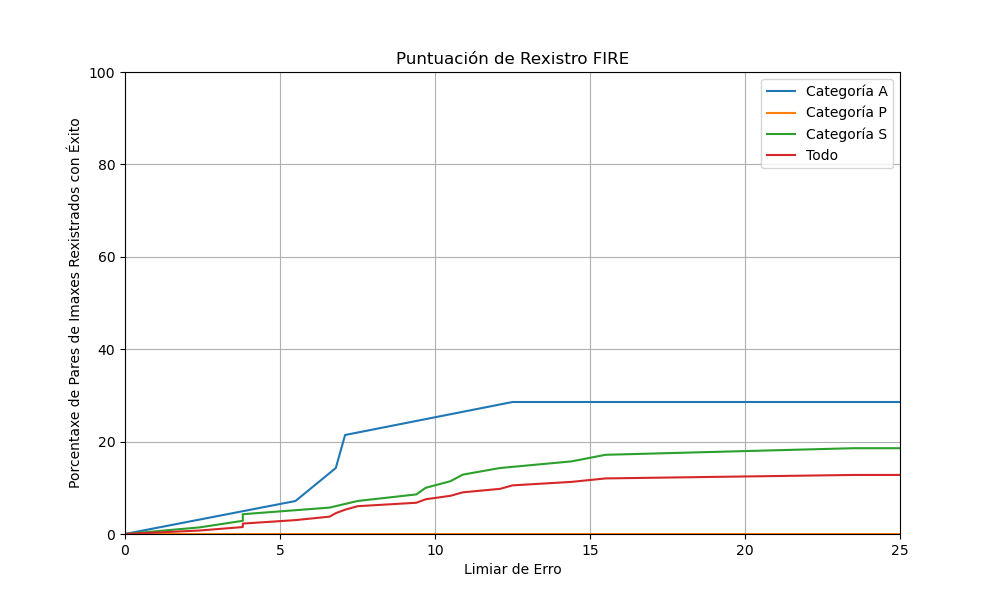
\includegraphics[width=\textwidth]{imaxes/FIRE_scores/fire_registration_score_ReLU.png}
        \caption{Métrica FIRE, función de activación ReLU}
        \label{fig:FIRE_relu}
    \end{subfigure}\hfill
    \begin{subfigure}[b]{0.5\textwidth}
        \centering
        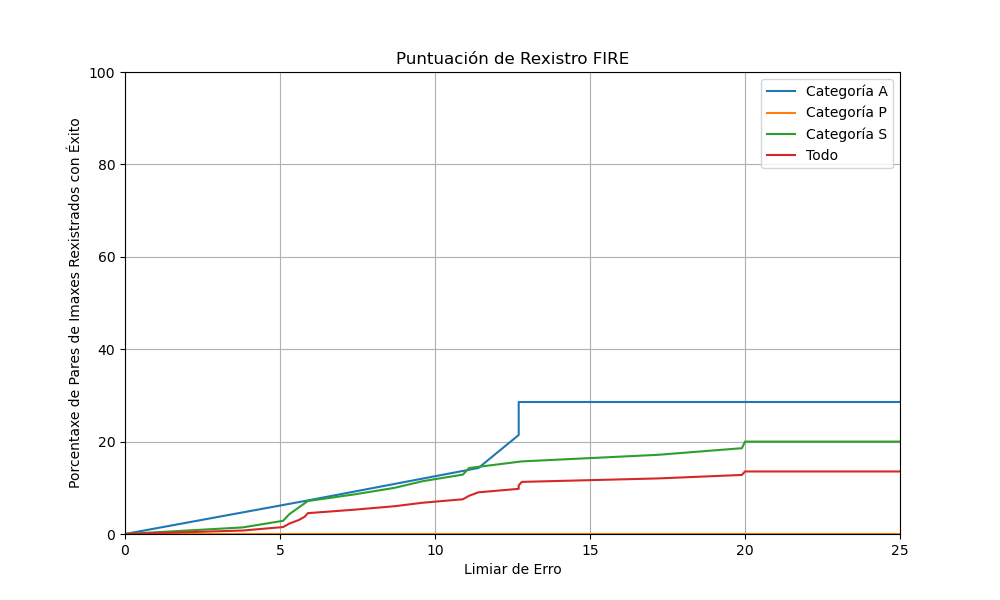
\includegraphics[width=\textwidth]{imaxes/FIRE_scores/fire_registration_scores_SIREN.png}
        \caption{Métrica FIRE, función de activación SIREN}
        \label{fig:FIRE_SIREN}
    \end{subfigure}
    \caption{Métricas dataset FIRE}
    \label{fig:FIRE_scores}
\end{figure}

\subsection{Descripción de los experimentos}
\label{subsec:Descrición dos experimentos}

\textbf{Experimentos iniciales:} En esta parte se realizarán experimentos para determinar unos valores aceptables para los parámetros de la red en el contexto de la imagen oftalmológica,
así como determinar su influencia en el rendimiento de la red.

\begin{itemize}
    \item \textbf{Función de pérdida:} Debido a las características únicas de las imágenes de retina, con variabilidad en iluminación y contraste, es crucial determinar qué función de pérdida es más robusta para esta tarea. Se compararon funciones basadas en píxeles (MSE, L1) con funciones basadas en características estructurales (NCC, SSIM) para determinar cuál captura mejor las correspondencias entre imágenes retinianas.
    \item \textbf{Resolución de la imagen:} Las imágenes de retina pueden tener resoluciones de hasta 2160×2160 píxeles, significativamente mayores que las imágenes de pulmón utilizadas originalmente por IDIR (512×512). Es necesario determinar si una mayor resolución mejora el rendimiento o si introduce ruido que perjudica el registro.
    \item \textbf{Regularización:} SIREN tiene un sesgo inherente hacia señales de alta frecuencia, lo que puede provocar sobreajuste. Se evalúa el impacto de diferentes términos de regularización (jacobiana, hiperelástica, energía de flexión) para determinar los valores óptimos que eviten deformaciones no realistas.
    \item \textbf{Tamaño de lote:} La densidad de puntos mostrados a la red puede ser crucial para el éxito del registro. Tamaños de lote mayores proporcionan más información por iteración, pero a un mayor coste computacional. Se investiga el equilibrio óptimo entre eficiencia y rendimiento.
\end{itemize}

\textbf{Estrategias de muestreo:} Las imágenes de retina tienen zonas con diferentes cantidades de información estructural (vasos sanguíneos, disco óptico vs. fondo uniforme). Se comparan estrategias de muestreo aleatorio, uniforme y ponderado por contenido para determinar si priorizar ciertas regiones mejora el registro.

\textbf{Inicialización:} La naturaleza no convexa de la función de pérdida puede hacer que diferentes inicializaciones converjan a mínimos locales distintos. Se implementó una lotería de inicialización para seleccionar la inicialización más prometedora basándose en la pérdida inicial.

\textbf{Ajuste dinámico del tamaño de lote:} Se teoriza que la red podría beneficiarse de aprender primero transformaciones globales con tamaños de lote pequeños y después refinar con mayores cantidades de puntos mostrados para capturar detalles locales.

\section{Ejemplos de registro}\label{sec:Ejemplos de registro}

Diferentes ejemplos de registro, tanto exitosos como fallidos, se pueden observar en la figura \ref{fig:reg_examples}.
La primera imagen corresponde con la imagen fija, la segunda corresponde con la imagen registrada, la tercera con la imagen móvil y la cuarta el campo de deformación aplicado a una rejilla cuadrada.

Se pueden observar los puntos de control, siendo los blancos los de la imagen fija, los verdes los de la imagen móvil y los azules los desplazados por la red.
\begin{figure}[tbp]
    \centering
    \begin{subfigure}[b]{0.45\textwidth}
        \centering
        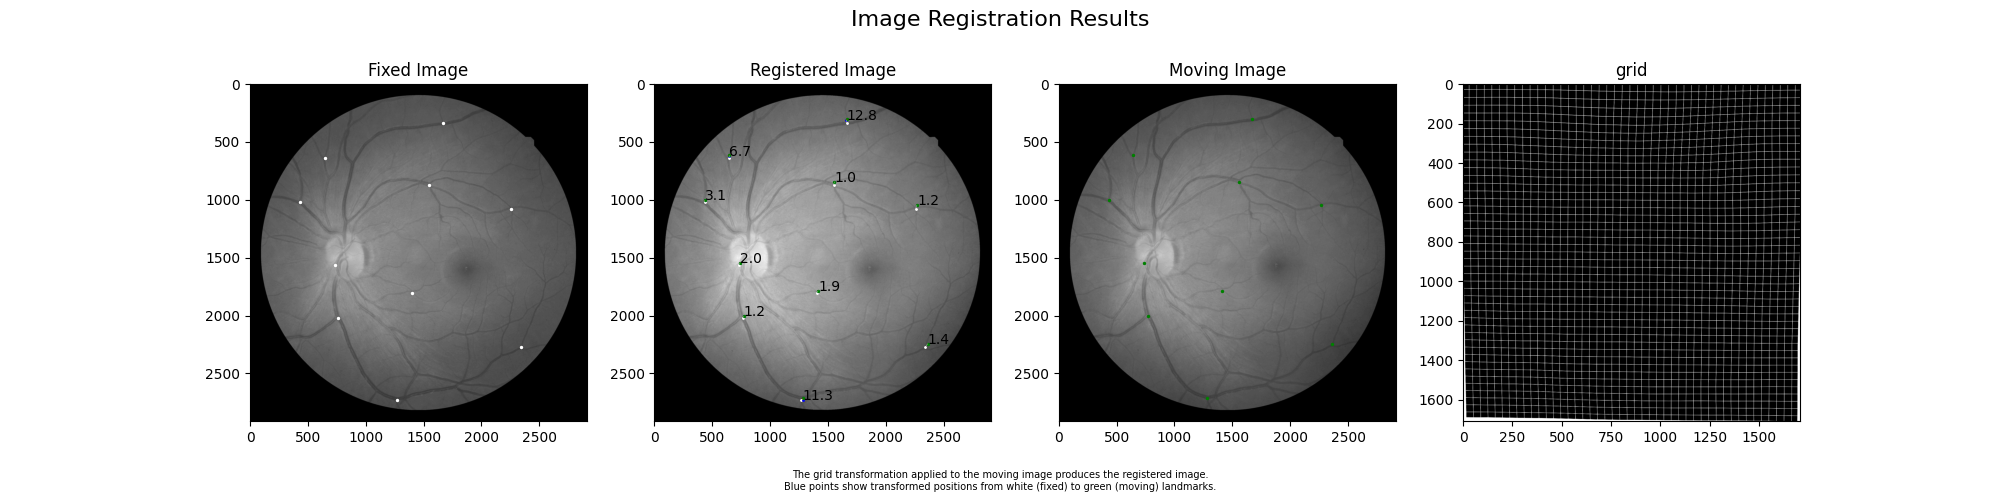
\includegraphics[width=\textwidth]{imaxes/reg_examples/FIRE_MLP_buena.png}
        \caption{Registro exitoso de un par de imágenes del dataset FIRE con la función de activación ReLU}
        \label{fig:reg_example_FIRE_MLP_buena}
    \end{subfigure}\hfill
    \begin{subfigure}[b]{0.45\textwidth}
        \centering
        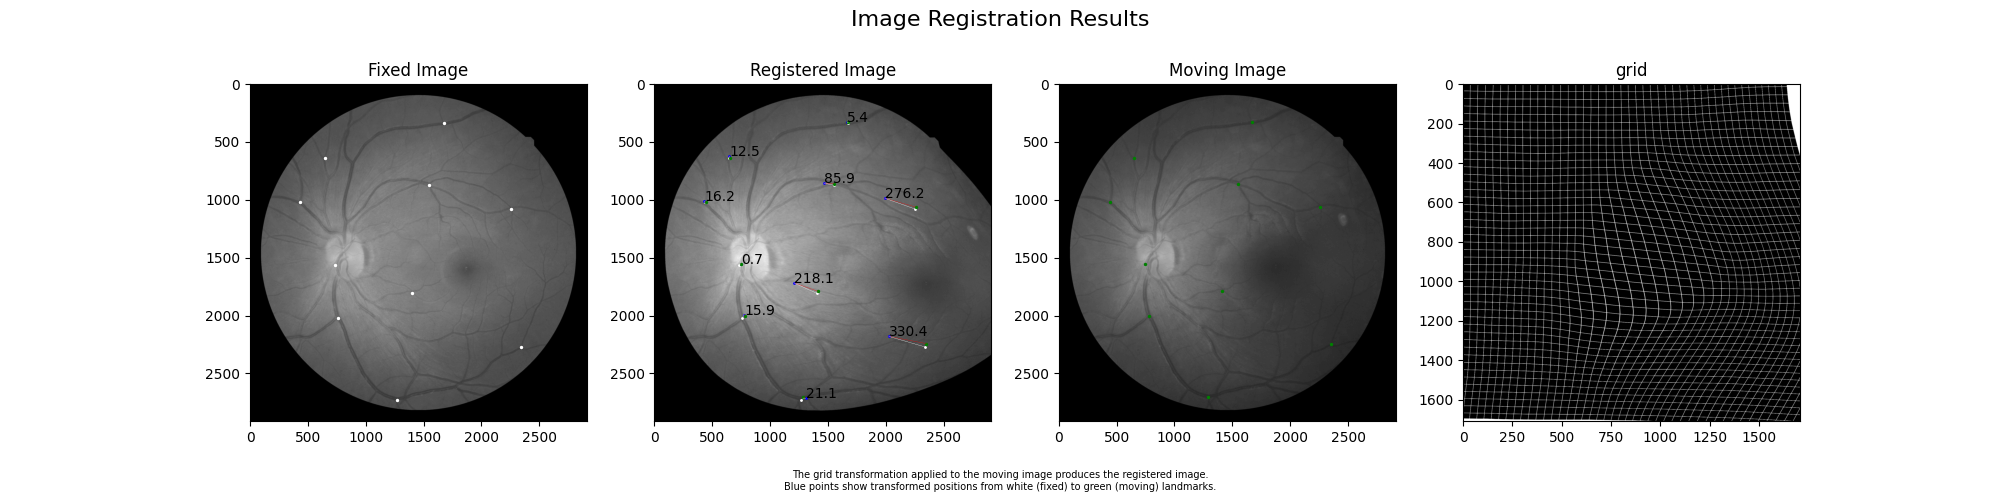
\includegraphics[width=\textwidth]{imaxes/reg_examples/FIRE_MLP_mala.png}
        \caption{Registro fallido de un par de imágenes del dataset FIRE con la función de activación ReLU}
        \label{fig:reg_example_FIRE_MLP_mala}
    \end{subfigure}

    \vskip\baselineskip

    \begin{subfigure}[b]{0.45\textwidth}
        \centering
        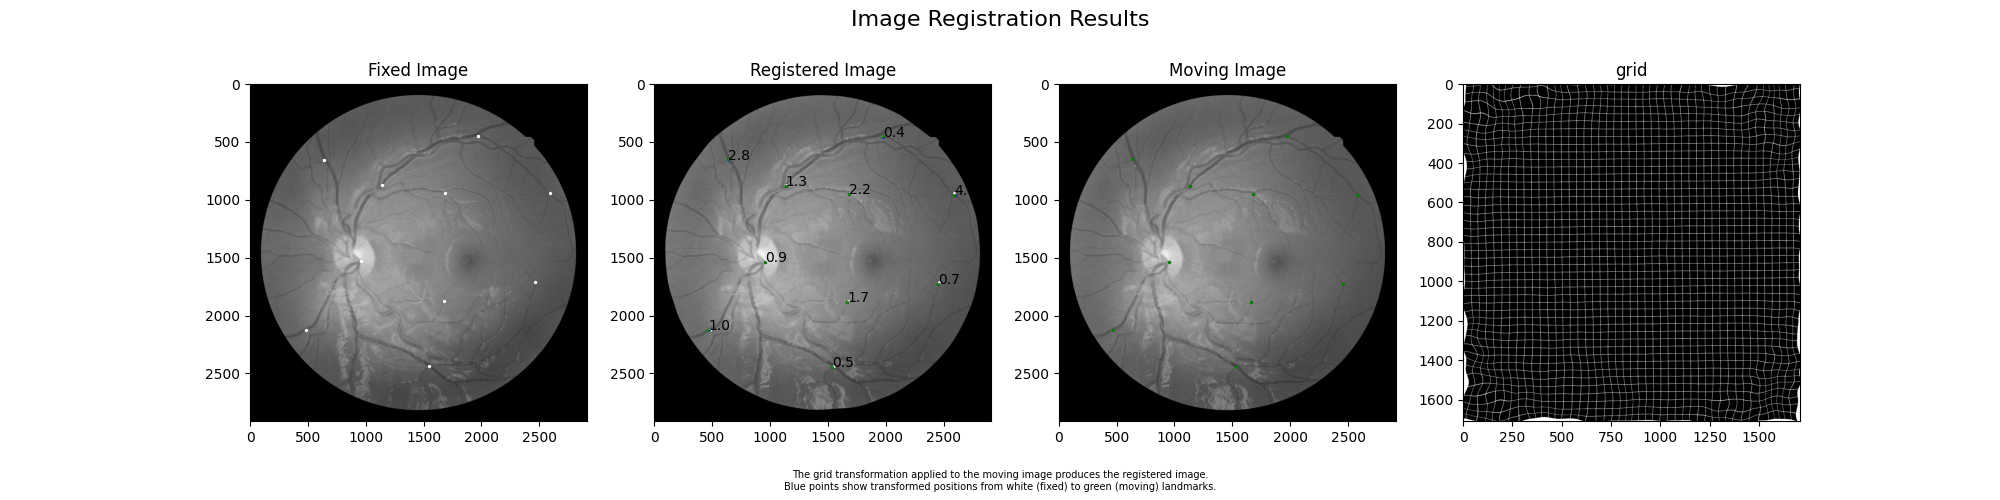
\includegraphics[width=\textwidth]{imaxes/reg_examples/FIRE_SIREN_buena.png}
        \caption{Registro exitoso de un par de imágenes del dataset FIRE con la función de activación SIREN}
        \label{fig:reg_example_FIRE_SIREN_buena}
    \end{subfigure}\hfill
    \begin{subfigure}[b]{0.45\textwidth}
        \centering
        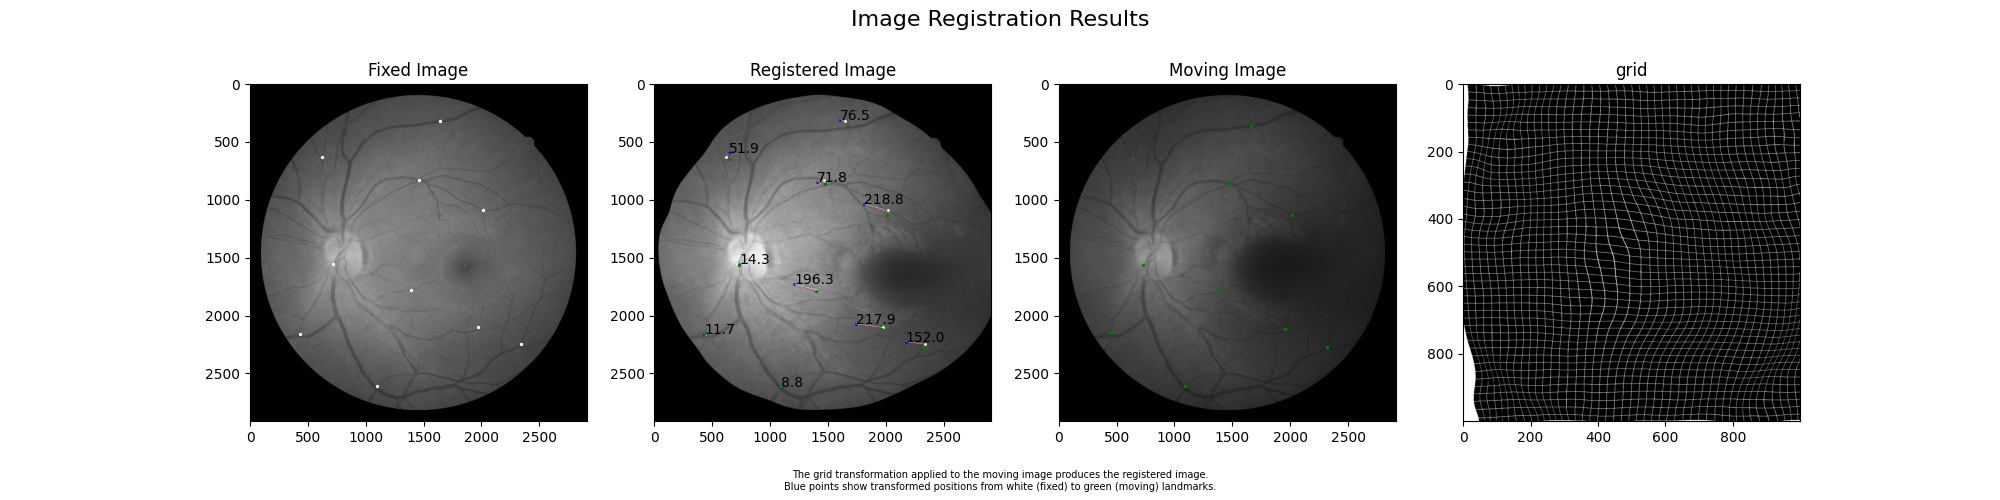
\includegraphics[width=\textwidth]{imaxes/reg_examples/FIRE_SIREN_mala.png}
        \caption{Registro fallido de un par de imágenes del dataset FIRE con la función de activación SIREN}
        \label{fig:reg_example_FIRE_SIREN_mala}
    \end{subfigure}

    \vskip\baselineskip

    \begin{subfigure}[b]{0.45\textwidth}
        \centering
        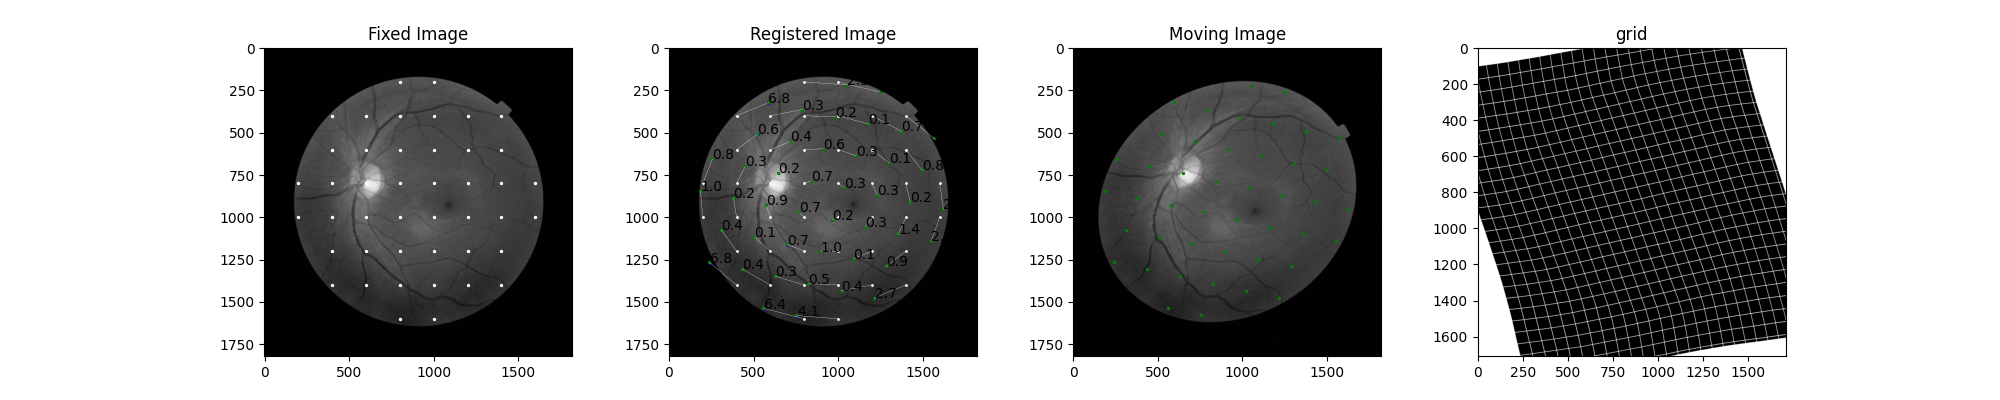
\includegraphics[width=\textwidth]{imaxes/reg_examples/RFMID_MLP_buena.png}
        \caption{Registro exitoso de un par de imágenes del dataset RFMID con la función de activación ReLU}
        \label{fig:reg_example_RFMID_MLP_buena}
    \end{subfigure}\hfill
    \begin{subfigure}[b]{0.45\textwidth}
        \centering
        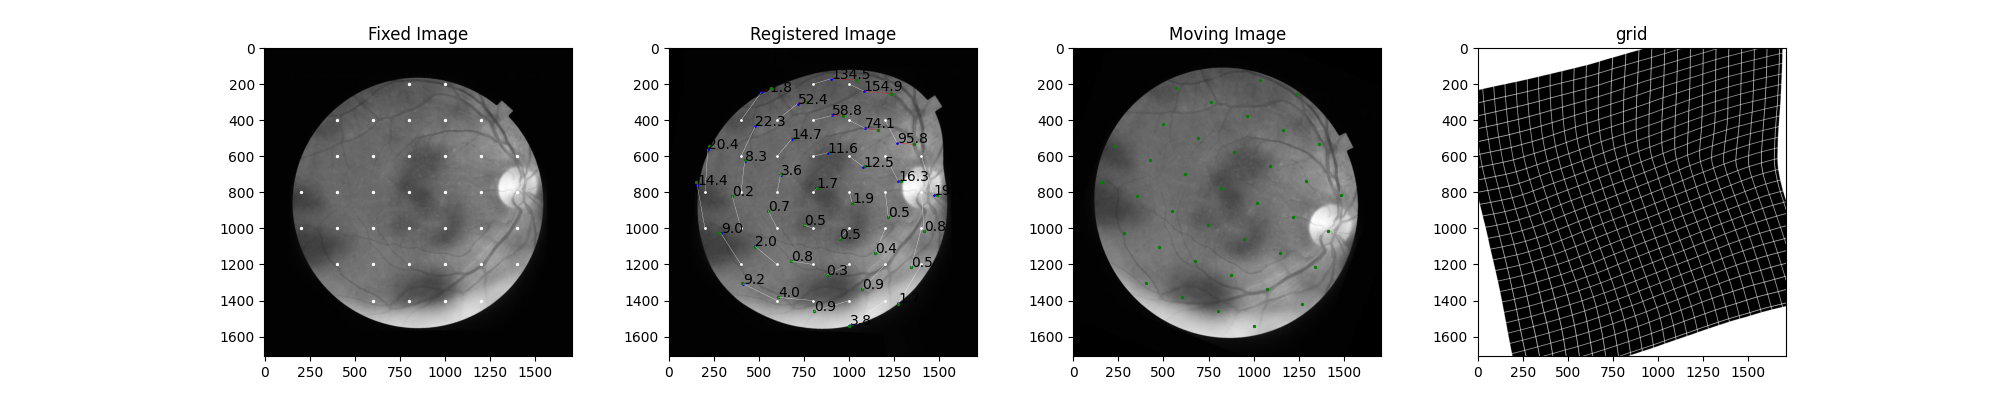
\includegraphics[width=\textwidth]{imaxes/reg_examples/RFMID_MLP_mala.png}
        \caption{Registro fallido de un par de imágenes del dataset RFMID con la función de activación ReLU}
        \label{fig:reg_example_RFMID_MLP_mala}
    \end{subfigure}

    \vskip\baselineskip

    \begin{subfigure}[b]{0.45\textwidth}
        \centering
        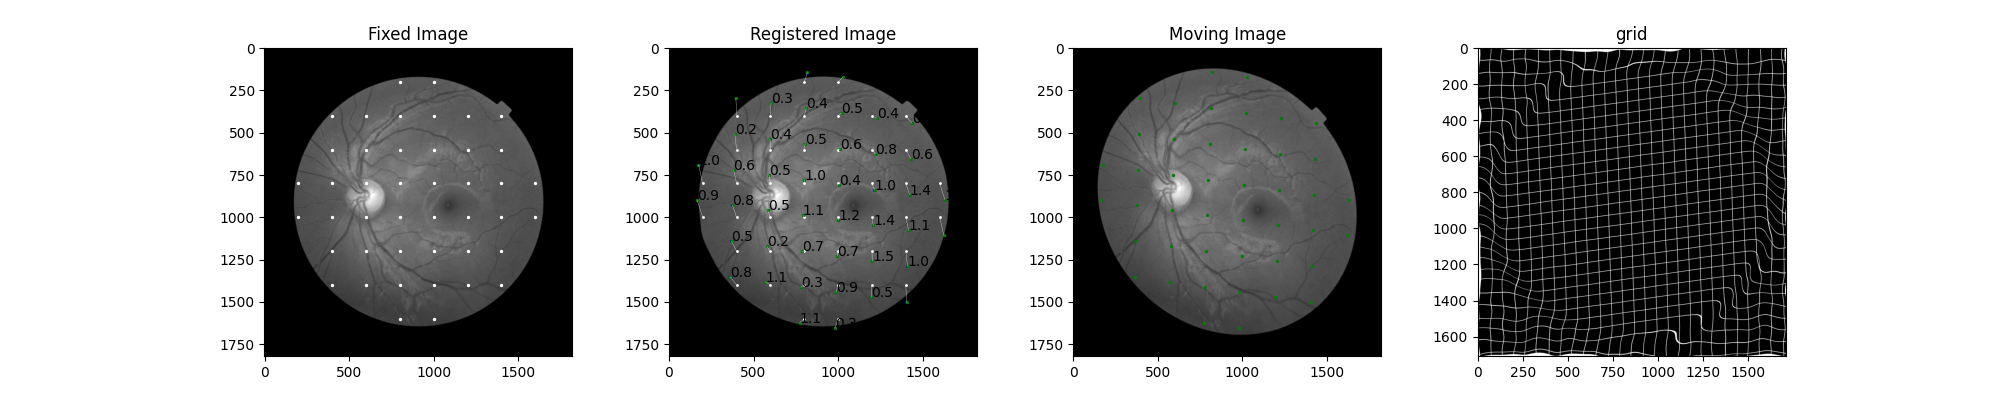
\includegraphics[width=\textwidth]{imaxes/reg_examples/RFMID_SIREN_buena.png}
        \caption{Registro exitoso de un par de imágenes del dataset RFMID con la función de activación SIREN}
        \label{fig:reg_example_RFMID_SIREN_buena}
    \end{subfigure}\hfill
    \begin{subfigure}[b]{0.45\textwidth}
        \centering
        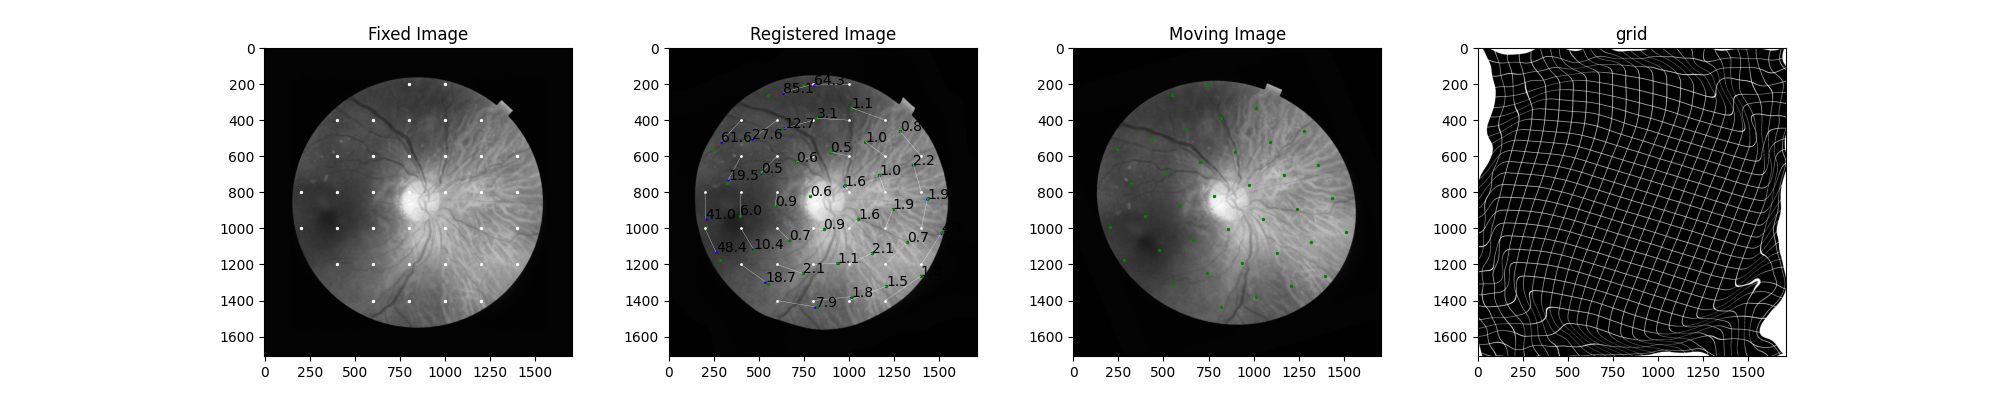
\includegraphics[width=\textwidth]{imaxes/reg_examples/RFMID_SIREN_mala.png}
        \caption{Registro fallido de un par de imágenes del dataset RFMID con la función de activación SIREN}
        \label{fig:reg_example_RFMID_SIREN_mala}
    \end{subfigure}

    \caption{Ejemplos de registro: combinaciones de dataset (FIRE/RFMID), función de activación (relu/SIREN) y éxito.}
    \label{fig:reg_examples}
\end{figure}

\section{Función de pérdida}
\label{sec:Función de pérdida}

\subsection{Planteamiento}
\label{subsec:Planteamiento-perda}

Las funciones de pérdida valoradas para este trabajo ya fueron explicadas en la sección \ref{subsubsec:Termos de Perda}.

Para determinar cuál es la función de pérdida más adecuada para la tarea de registro de retinas, se realizaron experimentos comparando el rendimiento de cada una sobre una muestra de imágenes de los datasets de FIRE y RFMID.
Ya que la red no es capaz de registrar con éxito gran parte de las imágenes en estas condiciones, se tomará la distancia media de todos los puntos como métrica de comparación.

\subsection{Resultados}
\label{subsec:Resultados-perda}

Se presenta en la figura \ref{fig:loss_functions_comparison} la comparación entre las diferentes funciones de pérdida.

\begin{figure}[tbp]
    \centering
    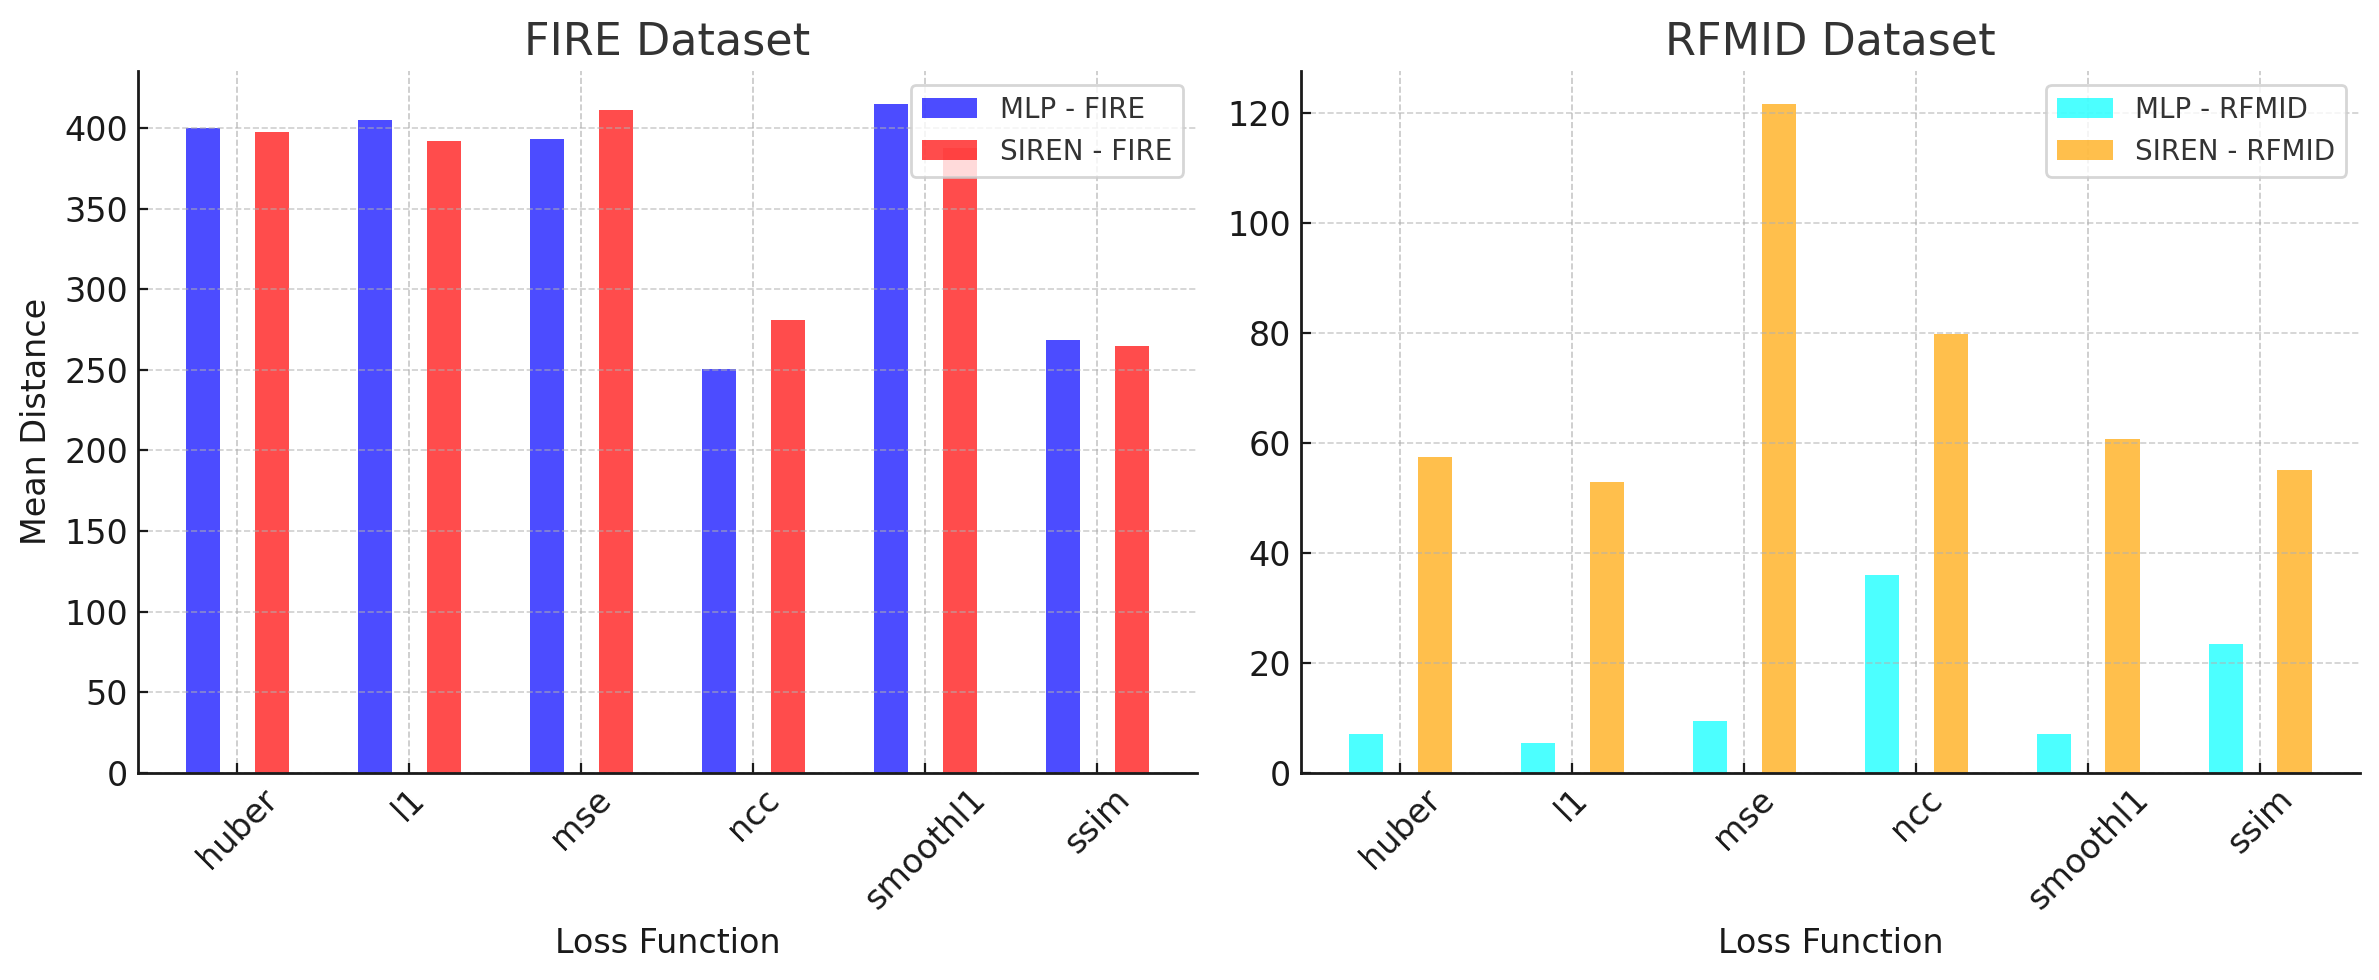
\includegraphics[width=1\textwidth]{imaxes/losstype.png}
    \caption{Comparación de diferentes funciones de pérdida sobre imágenes de FIRE y RFMID}
    \label{fig:loss_functions_comparison}
\end{figure}

\subsection{Discusión}
\label{subsec:Discusion-loss}

Se observa cómo las métricas que tienen en cuenta la estructura de la imagen (NCC, SSIM) tienden a dar mejores resultados que aquellas que no lo hacen (MSE, Huber, Smooth L1) con el dataset de FIRE, mientras que con RFMID ocurre lo contrario.
Esto puede deberse a que las imágenes reales de retina tienen una mayor variabilidad en la iluminación y contraste, por lo que las métricas que no tienen en cuenta la estructura de la imagen serán menos robustas a estas diferencias.
En el caso de RFMID, al ser imágenes sintéticas, la variabilidad en la iluminación y contraste es nula, lo que explica los mejores resultados de las métricas que no tienen en cuenta la estructura de la imagen.
De la misma forma, la función de activación Relu tiende a producir funciones predominantemente lineales, lo que se adapta mejor a las transformaciones realizadas en el dataset RFMID.

SSIM es menos robusta al ruido y sensible al tamaño de las secciones utilizadas, así como computacionalmente costosa. Además, tiene otro coste añadido ya que no es posible calcular SSIM tan solo comparando los puntos mostrados ya que utiliza ventanas deslizantes para evaluar luminancia, contraste y estructura.
Para utilizarla es necesario reconstruir la imagen en cada iteración lo que tiene un alto coste computacional.
En el caso de no reconstruir la imagen y utilizar los puntos mostrados directamente, esta métrica funciona igualmente pero con resultados ligeramente peores, ya que pierde toda su capacidad de capturar variaciones locales de luminancia, contraste y estructura, lo que se traduce en una función de pérdida global sin consideraciones locales.

\subsection{Conclusiones}
\label{subsec:Conclusions-loss}

En base a los resultados obtenidos, se pueden extraer las siguientes conclusiones:
\begin{itemize}
    \item Para el dataset FIRE, que contiene imágenes reales de retina con variabilidad en iluminación y contraste, las funciones de pérdida basadas en características estructurales como NCC y SSIM proporcionan resultados significativamente mejores.
    \item Para el dataset RFMID, que contiene imágenes con tan solo variación geométrica, las funciones de pérdida basadas en píxeles como L1 y Huber ofrecen mejores resultados.
    \item Se observa una diferencia sistemática entre los modelos Relu y SIREN, siendo los primeros más efectivos para el dataset RFMID, mientras que ambos muestran rendimientos comparables para FIRE.
\end{itemize}

\section{Resolución de la imagen}
\label{sec:Resolución de la imagen}

\subsection{Planteamiento}
\label{subsec:Planteamiento-resolution}

Para determinar cuál es la resolución más adecuada, se realizaron experimentos comparando el rendimiento de cada una sobre una muestra de imágenes de los datasets de FIRE y RFMID.
Debido a que la red no es capaz de registrar con éxito gran parte de las imágenes, se tomará la distancia media de todos los puntos como métrica de comparación.

La resolución de la imagen influye de forma directa en el resto de parámetros de la red.
Por ejemplo, un tamaño de lote de 1000 puntos en una imagen de 256x256 es una densidad de puntos mucho mayor que en una imagen de 1024x1024.

Además, la resolución de la imagen también influye en la capacidad de la red para aprender las transformaciones, ya que la información que recibe es más detallada.
Esto puede ser beneficioso si estos detalles contienen información relevante para la tarea de registro, pero también podría ser perjudicial si contienen una gran parte de ruido.

El tamaño de las imágenes también es una de las principales diferencias entre las imágenes de retina y las de pulmones utilizadas originalmente por IDIR, teniendo estas últimas de 512x512 mientras que las imágenes de los ojos cuentan con resoluciones de hasta 2160x2160.

\subsection{Resultados}\label{subsec:Resultados-resolution}

Se presenta en la figura \ref{fig:resoluciónchart} la comparación entre las diferentes resoluciones.

\begin{figure}[tbp]
    \centering
    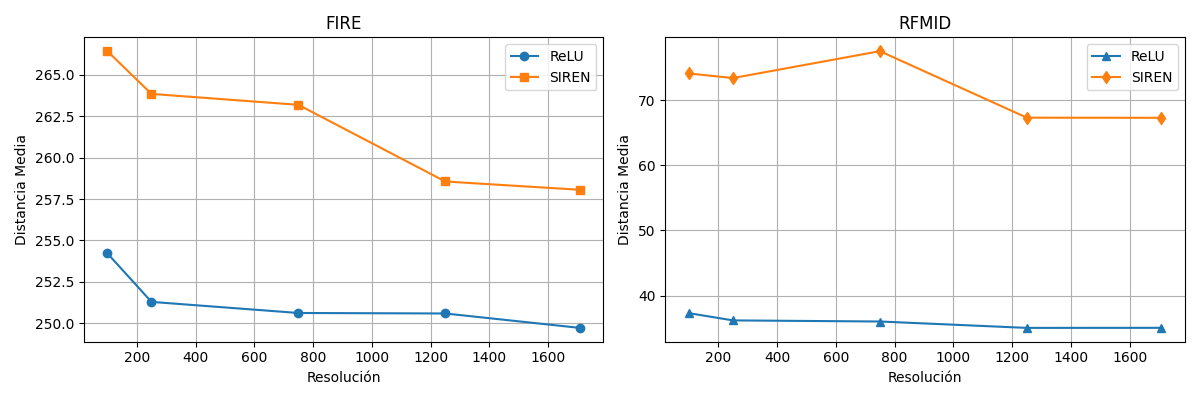
\includegraphics[width=1\textwidth]{imaxes/resolutionchart.png}
    \caption{Comparación de diferentes resoluciones de pérdida sobre imágenes de FIRE y RFMID. Menor distancia media es mejor.}
    \label{fig:resoluciónchart}
\end{figure}

\subsection{Discusión}
\label{subsec:Discusion-resolution}

Se puede observar cómo una mayor resolución tiende a dar ligeramente mejores resultados, pero a un coste computacional mayor.
Esto puede deberse a la precisión con la que se hace la evaluación más que a una mejor capacidad de la red para aprender las transformaciones, ya que las diferencias son muy pequeñas y consistentes entre los diferentes pares de imágenes.
Esto sugiere que la resolución no tiene un impacto significativo en el rendimiento de la red, y que la mayoría de la información relevante para la tarea de registro ya está capturada en resoluciones inferiores.

\subsection{Conclusiones}
\label{subsec:Conclusions-resolution}

Basándonos en los resultados obtenidos, podemos concluir que:

1. Resoluciones inferiores a 100×100 no capturan suficientes detalles de las estructuras vasculares retinianas para realizar un registro preciso, especialmente en imágenes reales del dataset FIRE.

2. Aumentar la resolución por encima de 1250x1250 no aporta beneficios significativos.

Para los experimentos subsiguientes, se adoptará una resolución estándar de 1250x1250 píxeles, que demostró proporcionar un buen balance entre rendimiento y eficiencia computacional.

\section{Regularización}
\label{sec:Regularización}

\subsection{Planteamiento}
\label{subsec:Planteamento-regularization}

Para determinar cuál es la cantidad de regularización óptima, se realizaron experimentos comparando el rendimiento de cada una sobre una muestra de imágenes de los datasets de FIRE y RFMID con las diferentes funciones de activación y diferentes grados de regularización.

El proceso de regularización ayuda a la red a evitar el sobreajuste, modificando el término de pérdida para penalizar las transformaciones poco realistas.
Las técnicas de regularización valoradas, que ya fueron explicadas en detalle en la sección \ref{subsubsec:Termos de regularización}

Los valores utilizados para cada tipo de regularización se ajustaron a partir de los utilizados originalmente por IDIR y comparado el impacto de cada uno de ellos sobre la función de pérdida, ya que la escala de cada uno de ellos es diferente.

En el anexo \ref{sec:Anexo regularization} se detalla una búsqueda más completa para explorar las relaciones entre los diferentes tipos de regularización.
En este apartado solo se presentarán los resultados de los experimentos realizados con la regularización hiperelástica, que se considera la más relevante para esta tarea.

\subsection{Resultados}
\label{subsec:Resultados-regularization}

La comparación entre los diferentes valores de regularización hiperelástica se presenta en la figura \ref{fig:barplot_hyper_reg_comparison}.

\begin{figure}[tbp]
    \centering
    \begin{subfigure}[b]{0.48\textwidth}
        \centering
        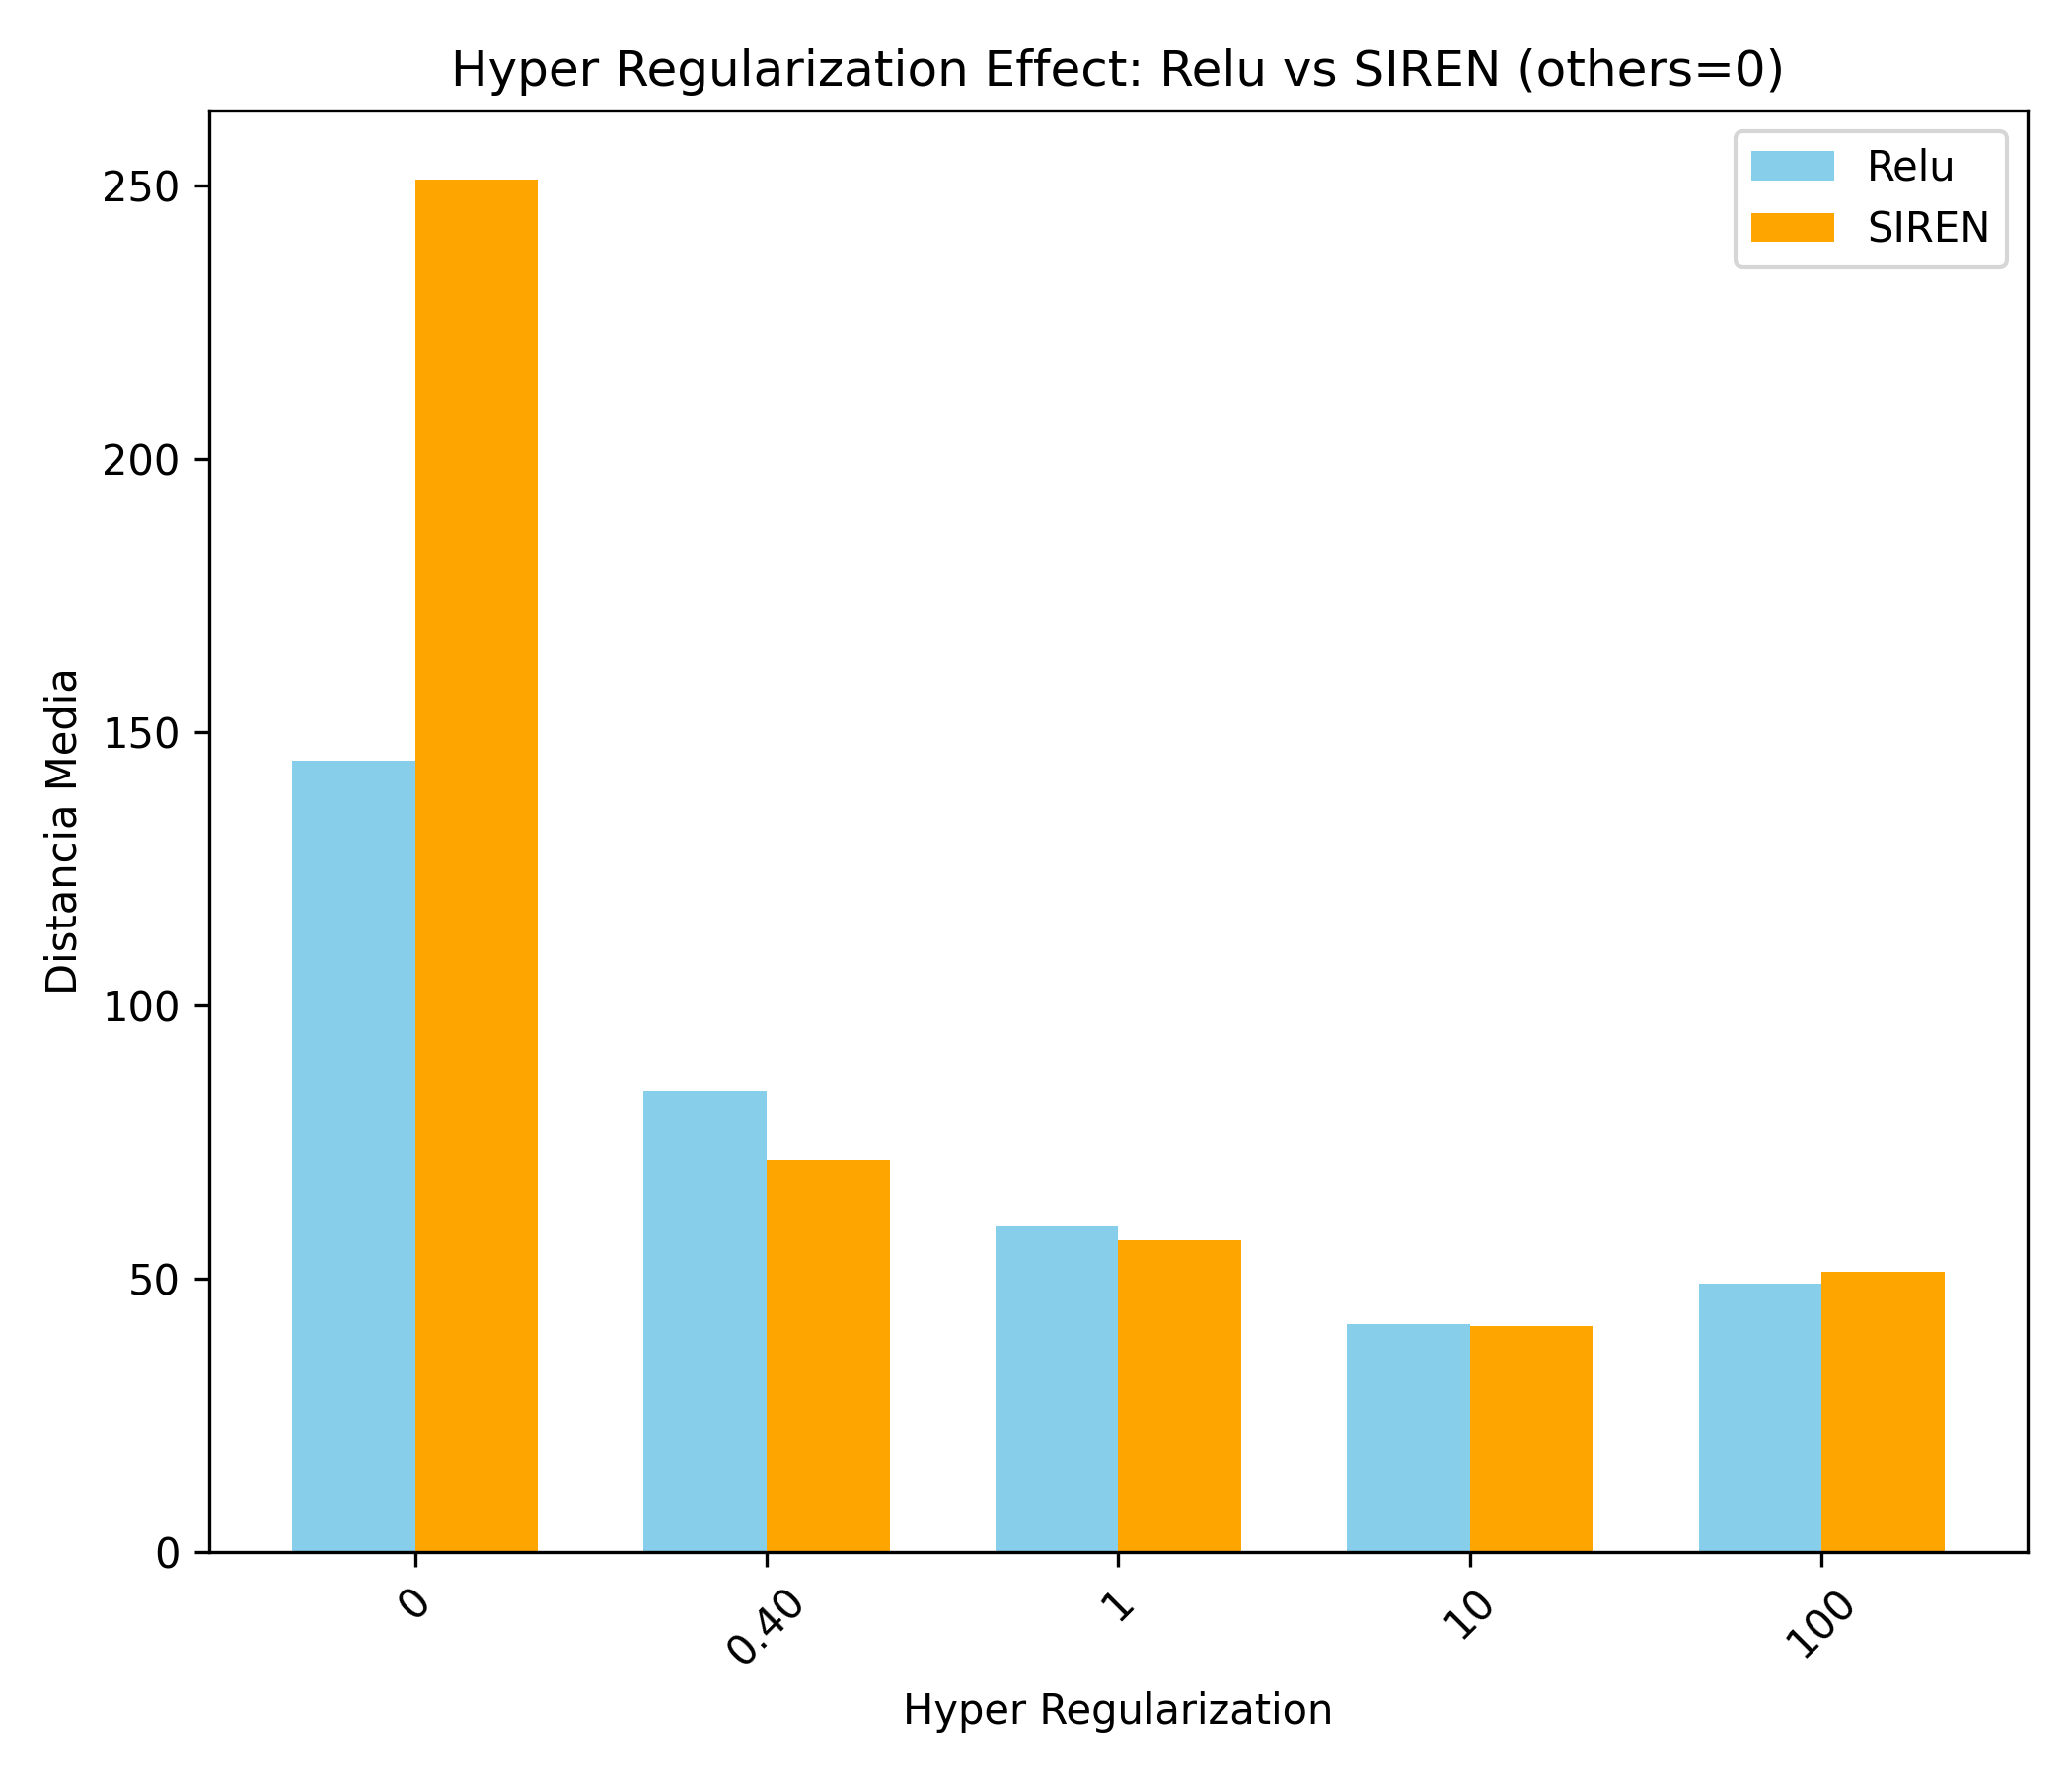
\includegraphics[width=\textwidth]{imaxes/reg_examples/barplot_hyper_reg_comparison_MLP_vs_SIREN_FIRE.png}
        \caption{Comparación de regularización hiperelástica en FIRE}
        \label{fig:barplot_hyper_reg_comparison_MLP_vs_SIREN_FIRE}
    \end{subfigure}\hfill
    \begin{subfigure}[b]{0.48\textwidth}
        \centering
        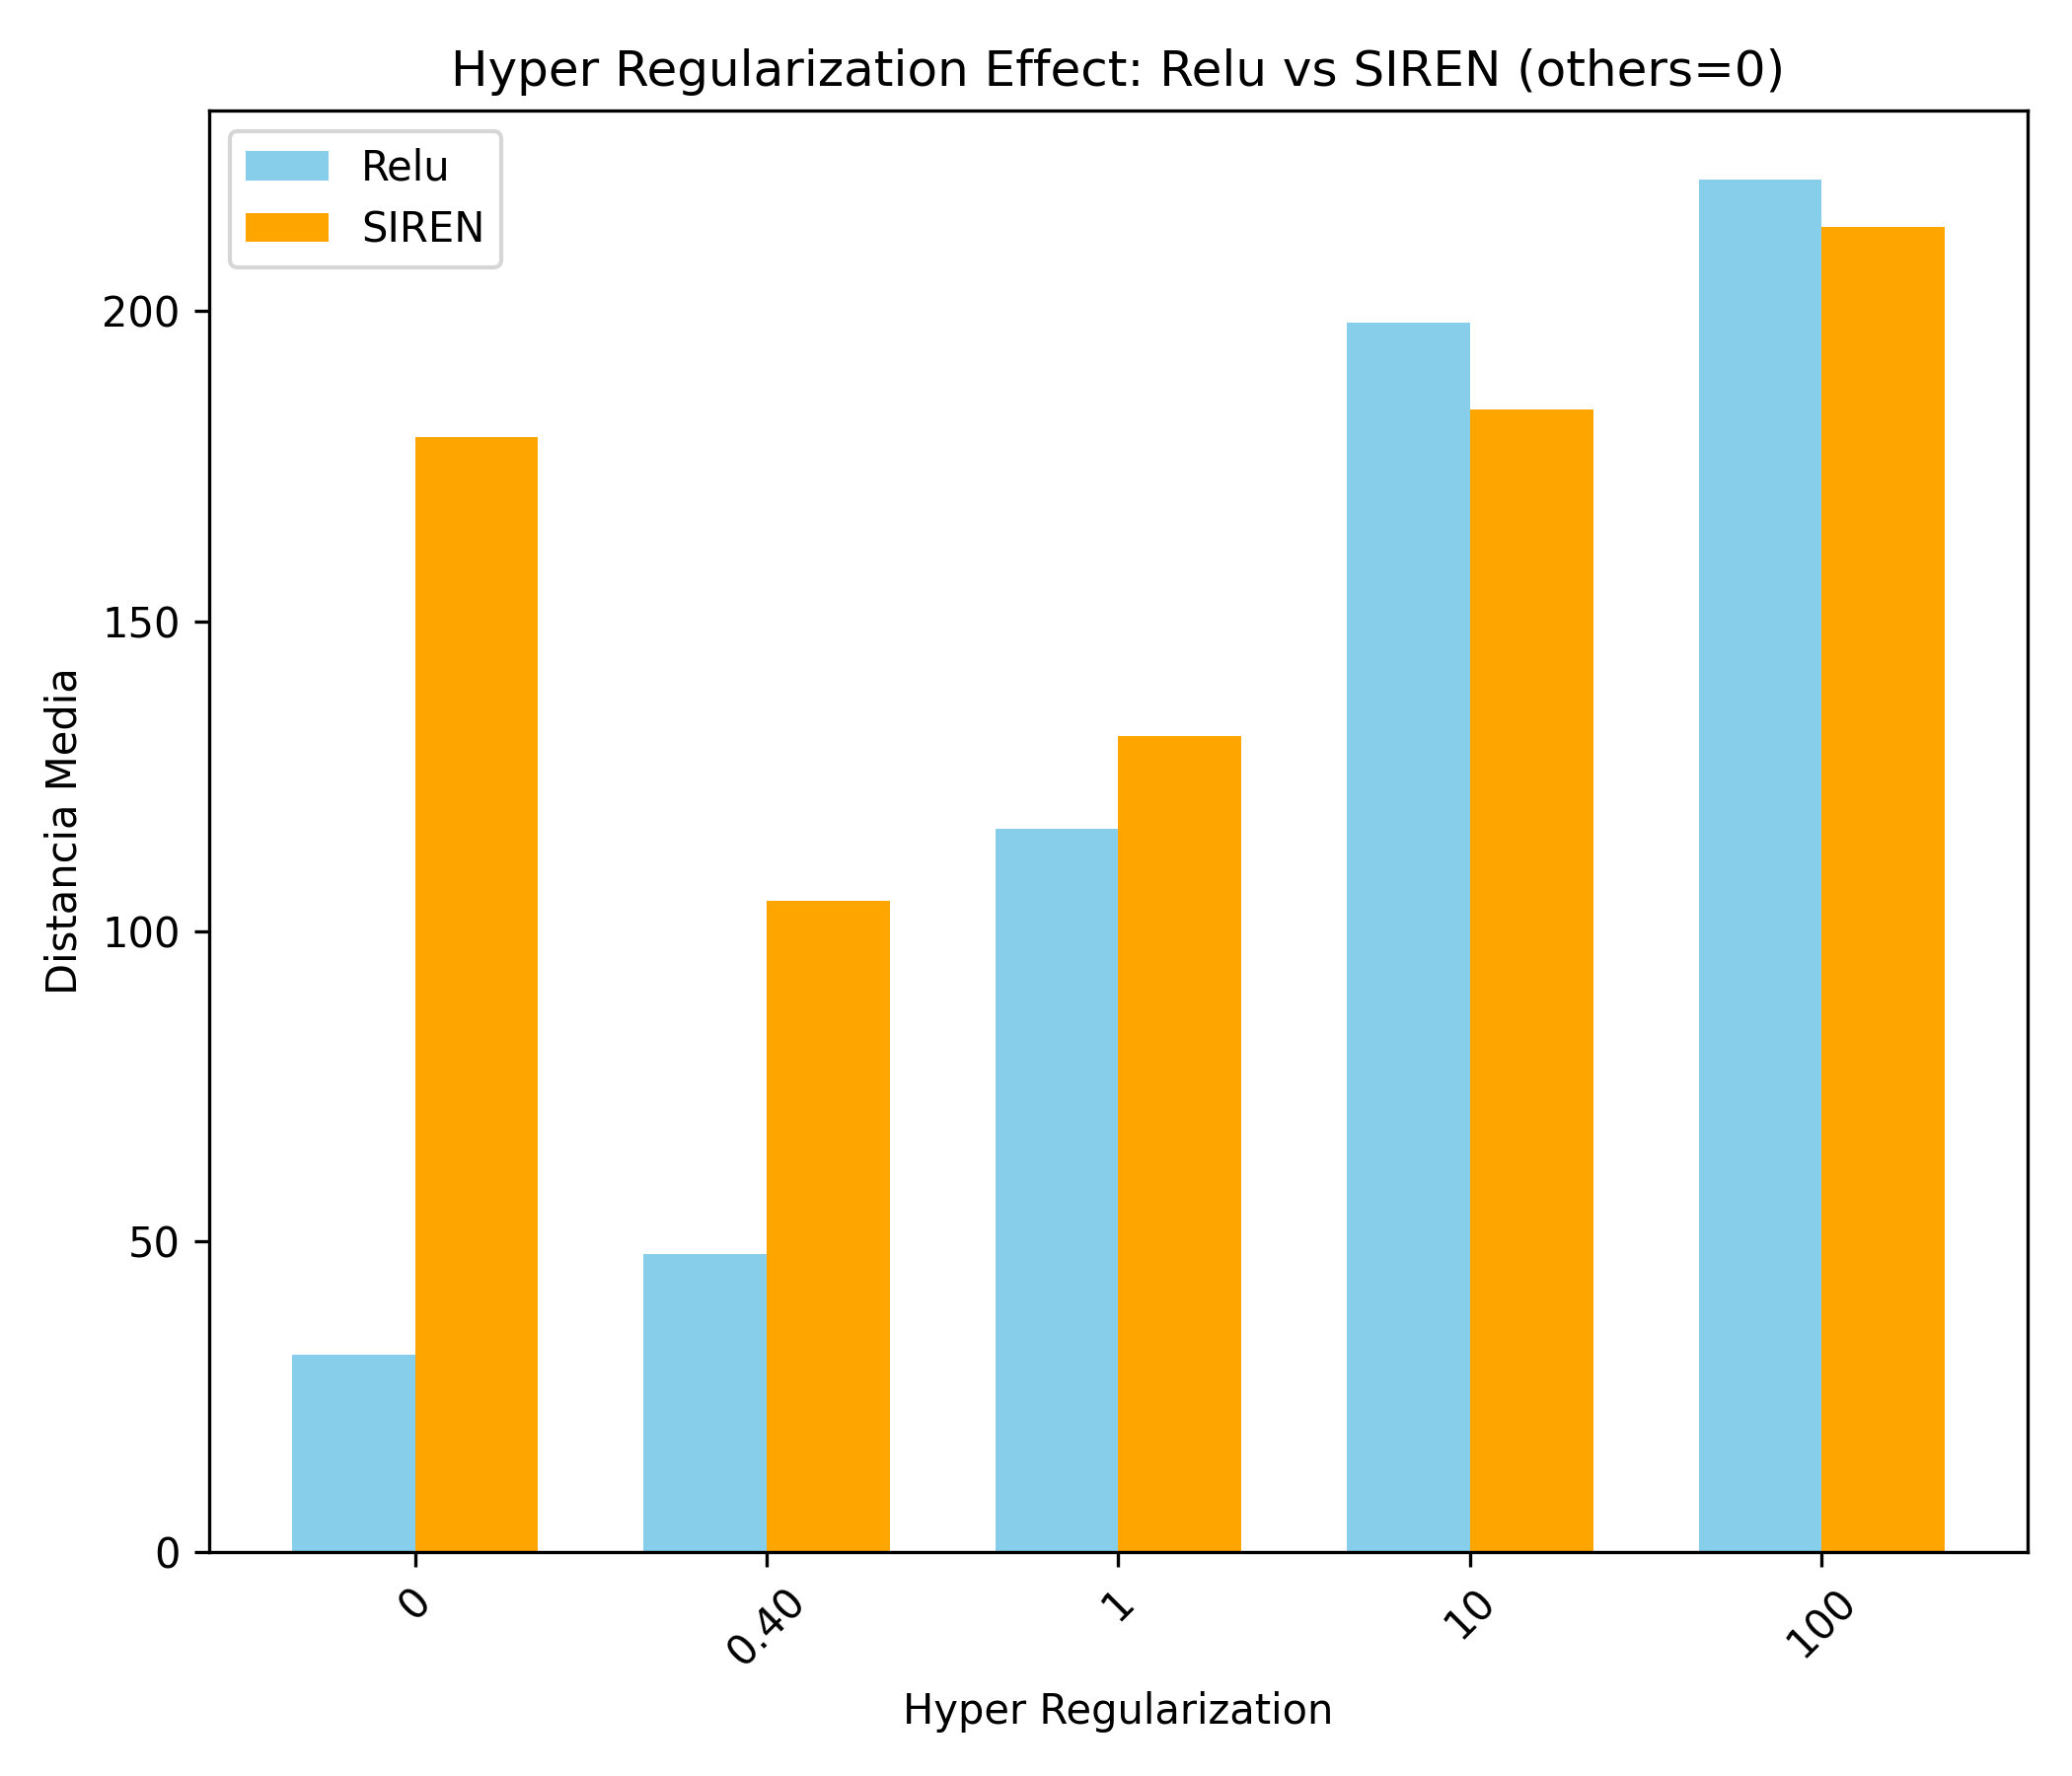
\includegraphics[width=\textwidth]{imaxes/reg_examples/barplot_hyper_reg_comparison_MLP_vs_SIREN_RFMID.png}
        \caption{Comparación de regularización hiperelástica en RFMID}
        \label{fig:barplot_hyper_reg_comparison_MLP_vs_SIREN_RFMID}
    \end{subfigure}
    \caption{Comparación del impacto de la regularización hiperelástica sobre los datasets FIRE y RFMID para modelos ReLU y SIREN}
    \label{fig:barplot_hyper_reg_comparison}
\end{figure}

\subsection{Discusión}
\label{subsec:Discusion-regularization}

Los resultados muestran que la regularización tiene un impacto significativo en el rendimiento de la red. Tanto la ausencia de regularización como la regularización excesiva resultan en rendimiento deficiente.
En la figura \ref{fig:regularization_examples} se pueden observar ejemplos de registros con ambos problemas.

\begin{figure}[tbp]
    \centering
    \begin{subfigure}[b]{0.45\textwidth}
        \centering
        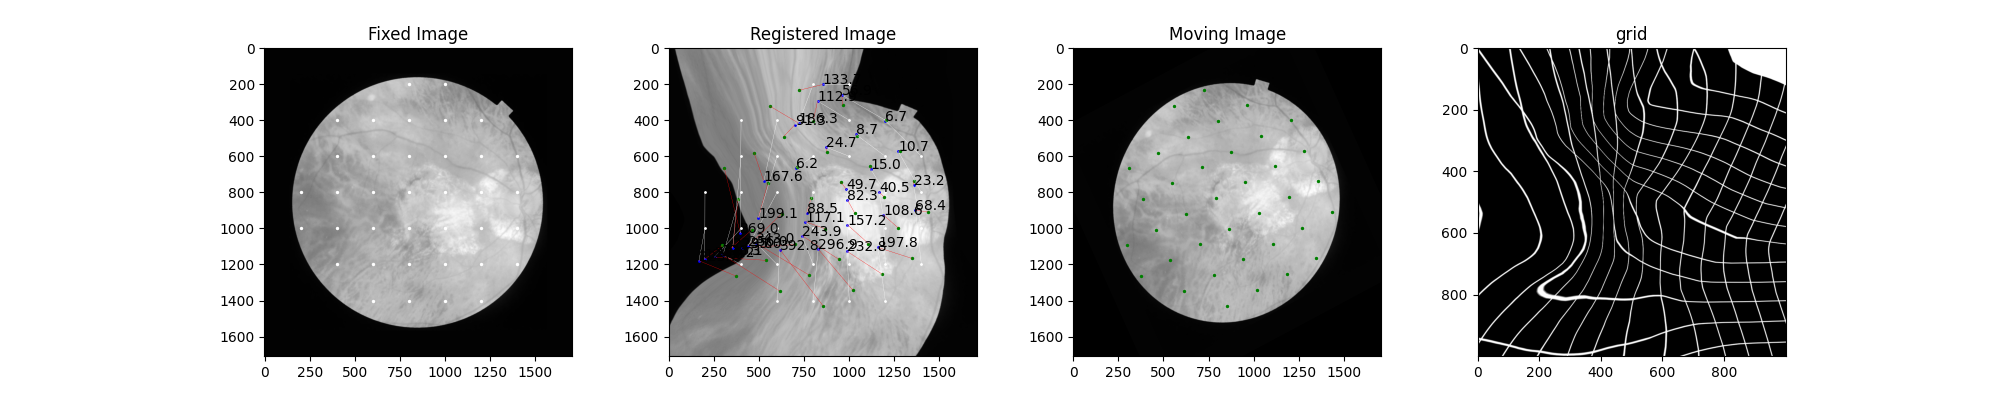
\includegraphics[width=\textwidth]{imaxes/reg_examples/no_reg_example.png}
        \caption{Ejemplo de registro con cero regularización, lo que provoca pliegues}
        \label{fig:no_reg_example}
    \end{subfigure}\hfill
    \begin{subfigure}[b]{0.45\textwidth}
        \centering
        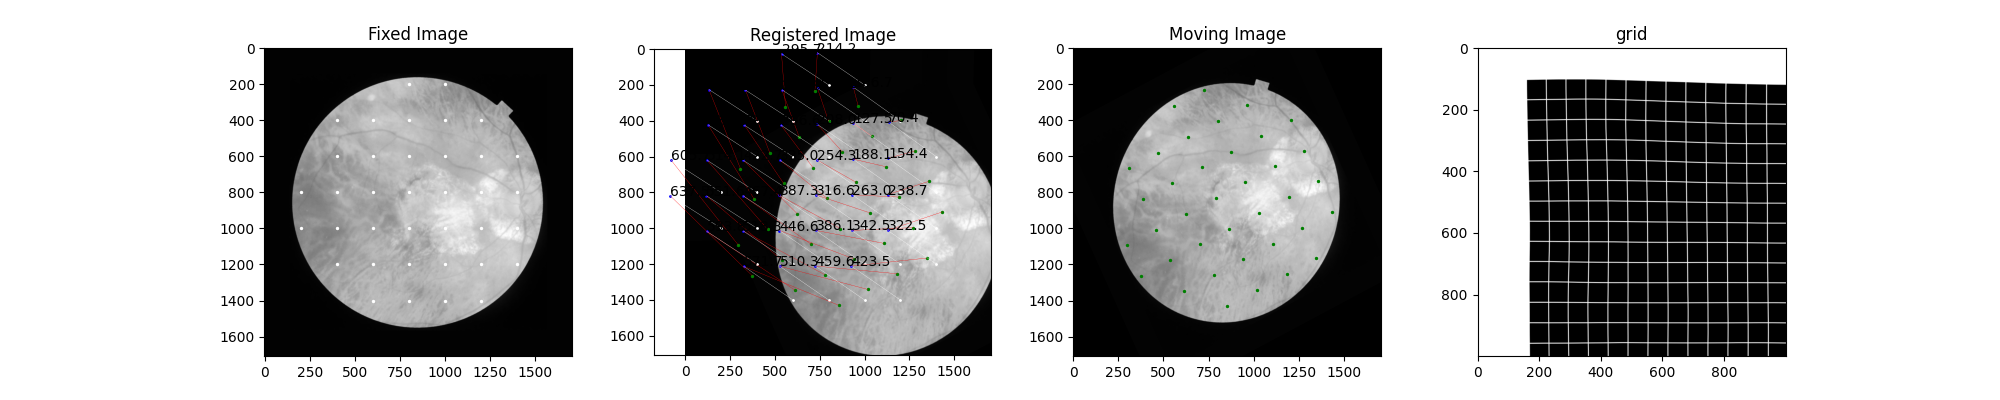
\includegraphics[width=\textwidth]{imaxes/reg_examples/too_much_reg_example.png}
        \caption{Ejemplo de registro con regularización excesiva, lo que evita que la red aprenda la transformación adecuada}
        \label{fig:too_much_reg_example}
    \end{subfigure}
    \caption{Ejemplos de registro con ausencia y exceso de regularización}
    \label{fig:regularization_examples}
\end{figure}

En los resultados se observa que Relu sigue dando mejores resultados que SIREN en el dataset RFMID, mientras que en el dataset FIRE ambos parecen tener un rendimiento similar.

La regularización óptima depende del tipo de registro que se está realizando. Los registros de transformaciones lineales (RFMID) se benefician de poca o ninguna regularización, mientras que los registros de transformaciones no lineales (FIRE) y con poca superposición se benefician de regularizaciones más elevadas.
Esto sugiere que la regularización es más relevante donde la red tiene que aprender transformaciones más complejas, ya que evita que caiga en mínimos locales no deseados.% \label{subsec:Conclusions-regularization}

En base a los resultados, se concluye que la regularización es un componente indispensable para el registro de retinas con redes implícitas. Su valor óptimo no es universal, sino que depende directamente de la complejidad de la transformación a aprender. Para deformaciones sencillas y lineales como las de RFMiD, una regularización mínima es suficiente, pero para los desafíos presentes en FIRE, con una mayor no linealidad, un término de regularización robusto es crucial para guiar la red hacia soluciones físicamente plausibles y evitar el sobreajuste. Se confirma también que los modelos SIREN, por su mayor capacidad para representar detalles de alta frecuencia, son más sensibles a la regularización y requieren valores generalmente más altos que los modelos ReLU para prevenir artefactos. La elección del coeficiente de regularización debe considerarse una decisión fundamental, adaptada tanto a la naturaleza del problema de registro como a la arquitectura de la red empleada.

\section{Tamaño de lote}
\label{sec:Tamaño de lote}

\subsection{Planteamiento}
\label{subsec:Planteamento-batchsize}

A lo largo de los experimentos realizados, el análisis cualitativo reveló que el tamaño de lote es uno de los parámetros que más impacto tiene en el rendimiento de la red.

De ahora en adelante dividimos el conjunto de datos de RFMID en varios subconjuntos según la dificultad de la transformación, como detallado en la sección \ref{subsec:Avaliación Cuantitativa}.

De esta forma podemos comparar el rendimiento de la red en diferentes subconjuntos de imágenes, y determinar si el rendimiento de la red es consistente entre ellos.

En los experimentos con el dataset FIRE, se decidió limitarse a la categoría S, ya que es la que mayor número de ejemplos tiene y tiene un mayor grado de superposición entre las imágenes, lo que facilita la tarea de registro.
Además, ya que la red sí que es capaz de registrar correctamente las imágenes de los subconjuntos más sencillos, utilizaremos la métrica de FIRE para medir el porcentaje de imágenes registradas correctamente.

\subsection{Resultados}
\label{subsec:Resultados-batchsize}

En las figuras \ref{fig:batch_size_comparison_relu_rfmid} y \ref{fig:batch_size_comparison_siren_rfmid} se pueden observar los resultados de la experimentación con el dataset RFMID a distintas dificultades y con distintos tamaños de lote.

\begin{figure}[tbp]
    \centering
    \begin{subfigure}[b]{0.5\textwidth}
        \centering
        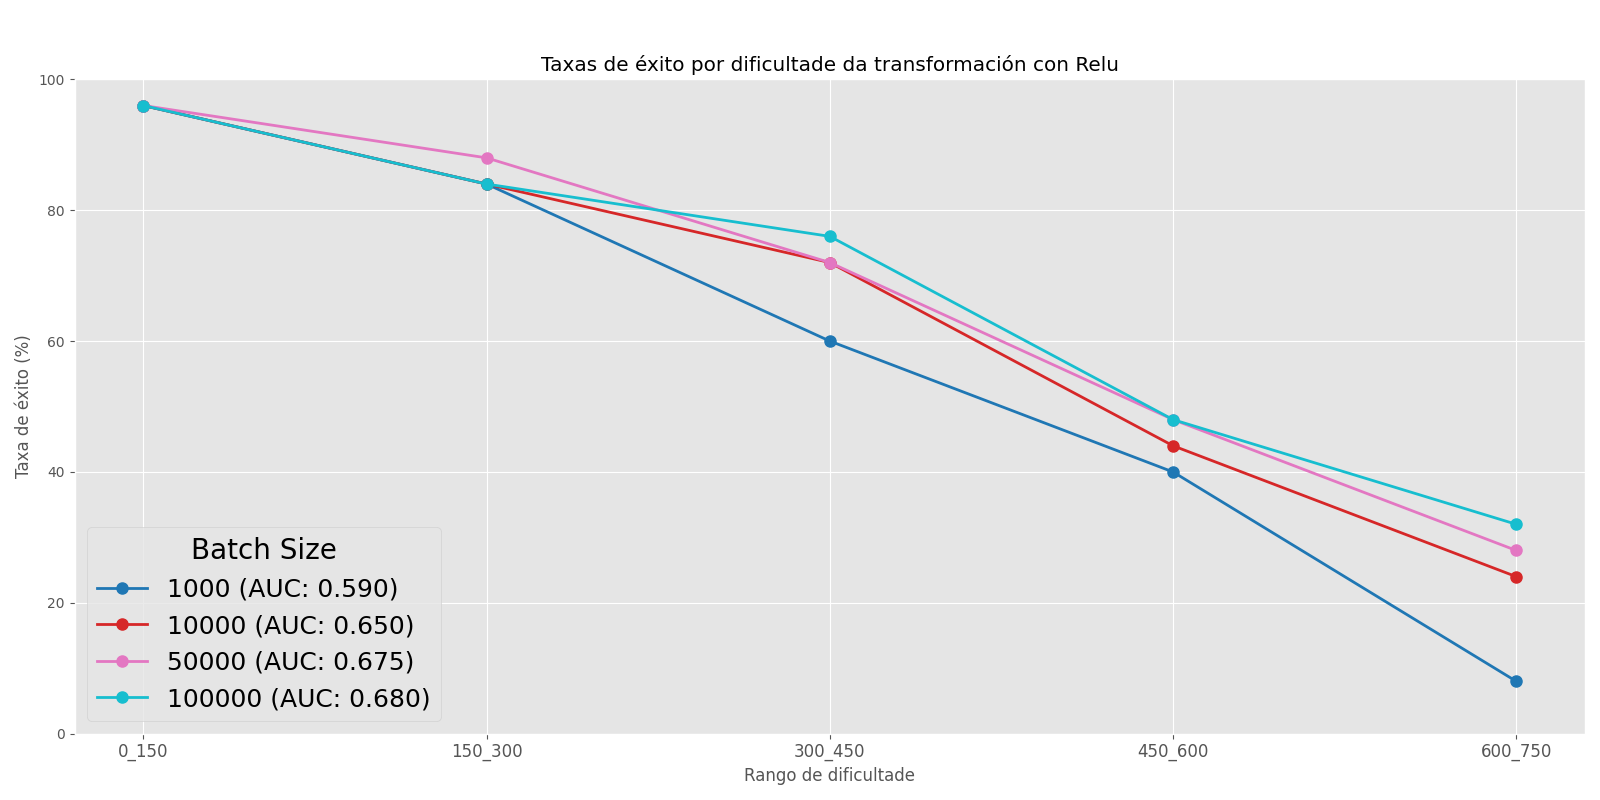
\includegraphics[width=\textwidth]{imaxes/batchsize/experiment_plot_RFMID_bs_relu.png}
        \caption{Función de activación ReLU}
        \label{fig:batch_size_comparison_relu_rfmid}
    \end{subfigure}\hfill
    \begin{subfigure}[b]{0.5\textwidth}
        \centering
        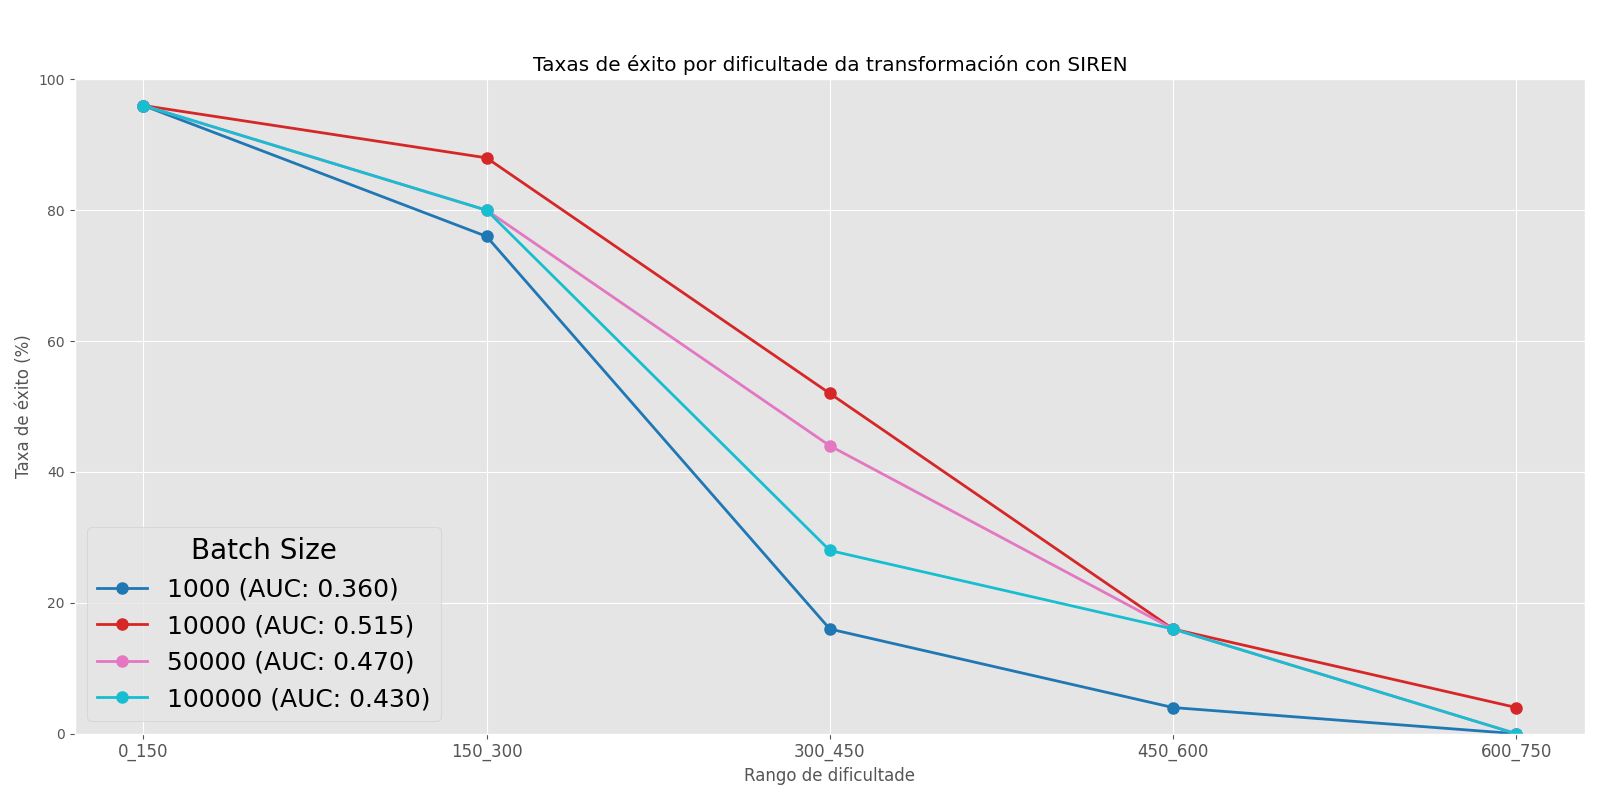
\includegraphics[width=\textwidth]{imaxes/batchsize/experiment_plot_RFMID_bs_siren.png}
        \caption{Función de activación SIREN}
        \label{fig:batch_size_comparison_siren_rfmid}
    \end{subfigure}
    \caption{Comparación del rendimiento de la red con diferentes tamaños de lote sobre imágenes del dataset RFMID, mostrando el porcentaje de registros exitosos para cada umbral de error.}
    \label{fig:batch_size_comparisons_rfmid}
\end{figure}

Con esta nueva división del dataset, también se realizó la evaluación por el método de evaluación de FIRE, que se puede ver en las figuras \ref{fig:FIRERFMID_relu} y \ref{fig:FIRERFMID_SIREN}.

\begin{figure}[tbp]
    \centering
    \begin{subfigure}[b]{0.5\textwidth}
        \centering
        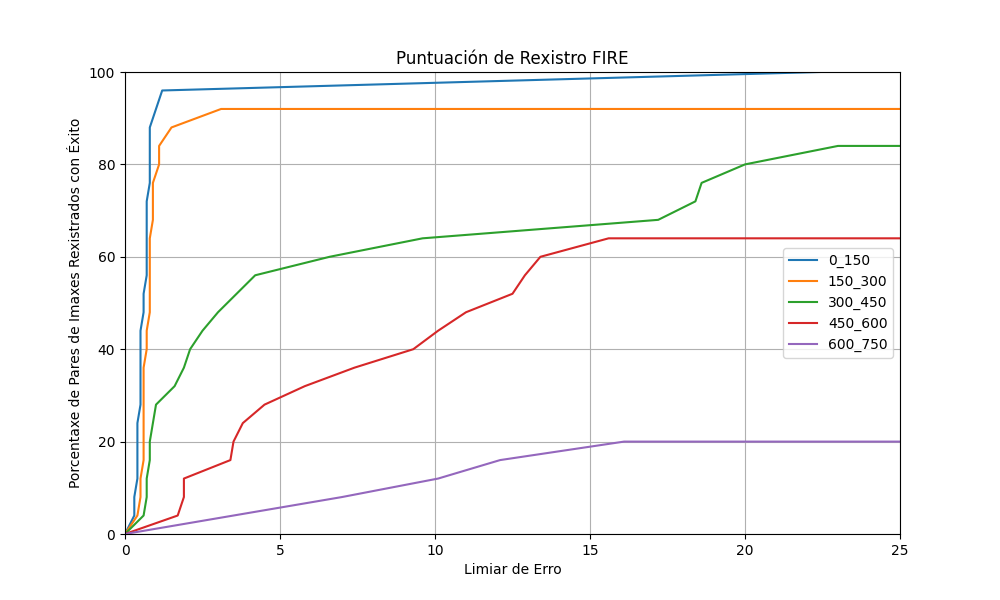
\includegraphics[width=\textwidth]{imaxes/FIRE_scores/fire_registration_scores_RFMID_MLP.png}
        \caption{Métrica FIRE con la función de activación ReLU}
        \label{fig:FIRERFMID_relu}
    \end{subfigure}\hfill
    \begin{subfigure}[b]{0.5\textwidth}
        \centering
        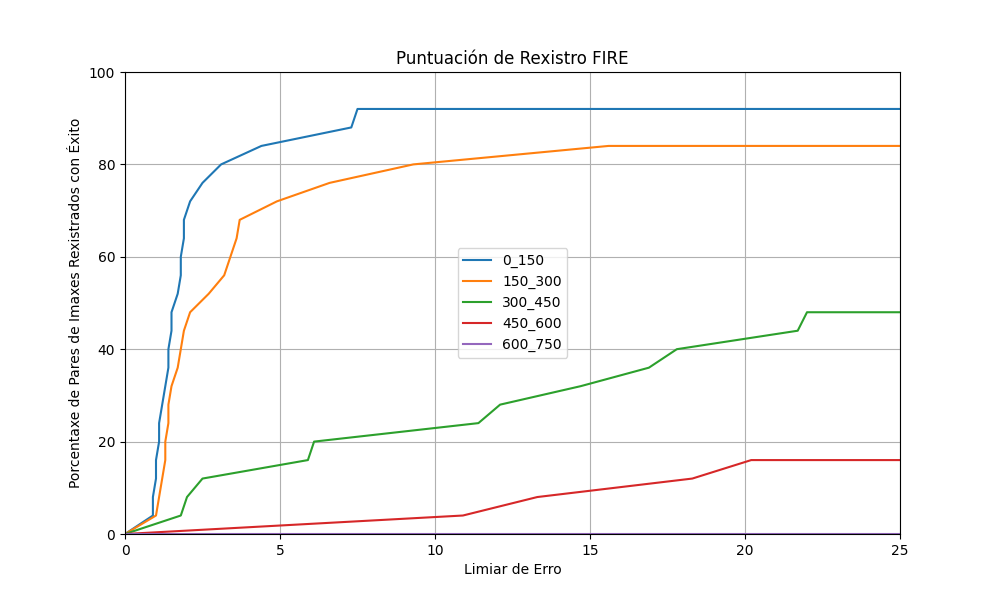
\includegraphics[width=\textwidth]{imaxes/FIRE_scores/fire_registration_scores_RMIFD_SIREN.png}
        \caption{Métrica FIRE con la función de activación SIREN}
        \label{fig:FIRERFMID_SIREN}
    \end{subfigure}
    \caption{Comparación del rendimiento de la red con diferentes tamaños de lote sobre imágenes del dataset FIRE}
    \label{fig:FIRERFMID_scores}
\end{figure}

En las figuras \ref{fig:batch_size_comparison_relu} y \ref{fig:batch_size_comparison_siren} se muestran los resultados de la experimentación con el dataset FIRE.

\begin{figure}[tbp]
    \centering
    \begin{subfigure}[b]{0.5\textwidth}
        \centering
        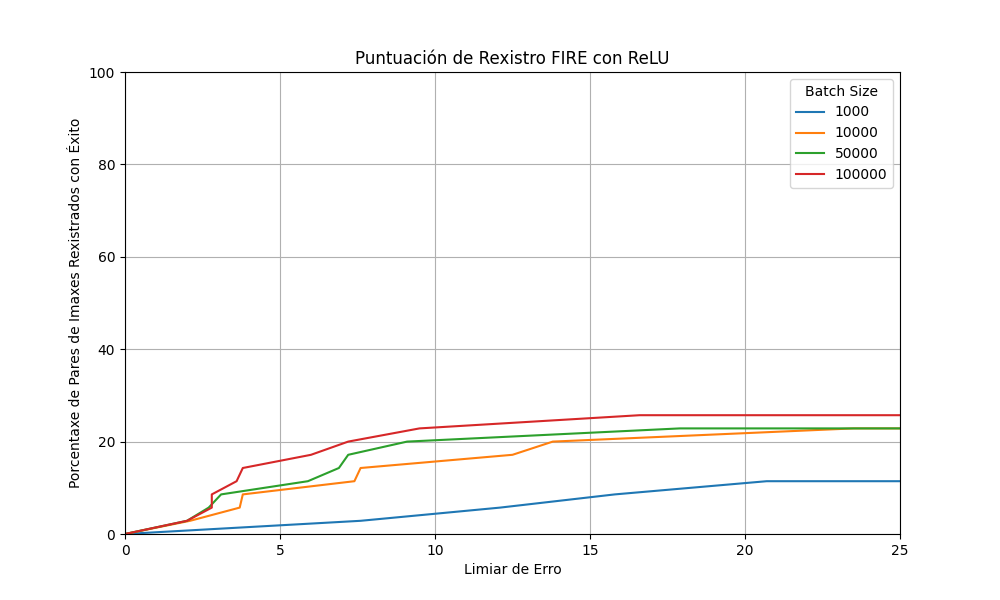
\includegraphics[width=\textwidth]{imaxes/batchsize/fire_registration_scores_bs_relu_S.png}
        \caption{Función de activación ReLU}
        \label{fig:batch_size_comparison_relu}
    \end{subfigure}\hfill
    \begin{subfigure}[b]{0.5\textwidth}
        \centering
        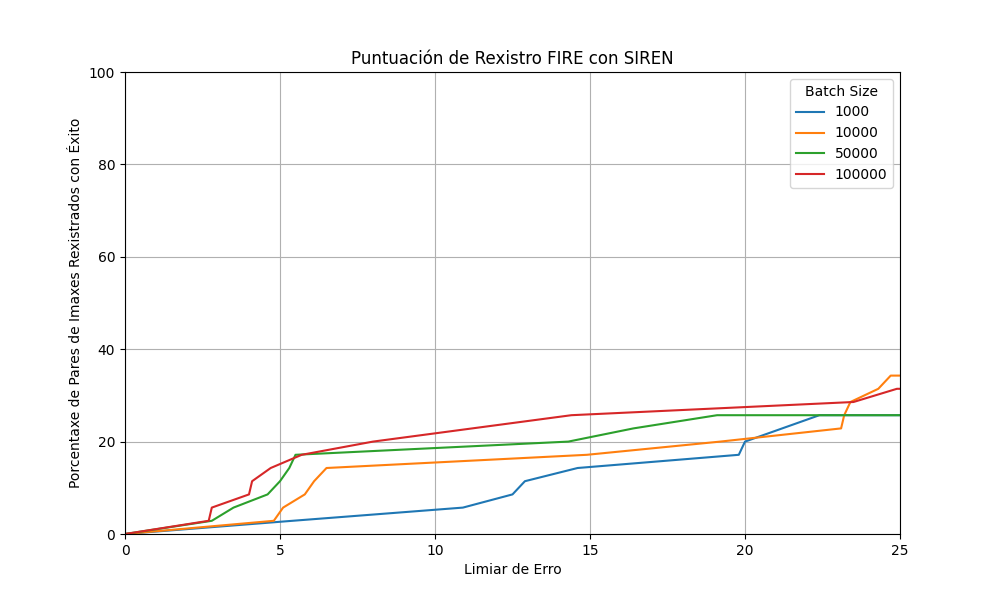
\includegraphics[width=\textwidth]{imaxes/batchsize/fire_registration_scores_bs_siren_S.png}
        \caption{Función de activación SIREN}
        \label{fig:batch_size_comparison_siren}
    \end{subfigure}
    \caption{Comparación del rendimiento de la red con diferentes tamaños de lote sobre imágenes de la categoría S del dataset FIRE}
    \label{fig:batch_size_comparisons_fire}
\end{figure}

\subsection{Discusión}
\label{subsec:Discusion-batchsize}

Se observa que las redes con la función de activación ReLU tienden a tener un rendimiento mucho mejor que las con la función de activación SIREN. Esto puede explicarse ya que las deformaciones artificiales que se aplican en las imágenes del dataset RFMID son lineales, y la función de activación ReLU es adecuada para este tipo de transformaciones.

También parece que el tamaño de lote es relevante, especialmente el cambio entre 1000 y 10000, mientras que valores mayores (50000, 100000) no parecen tener tanto impacto, aunque sí un mayor coste computacional.

Mientras que la red es capaz de registrar correctamente consistentemente las imágenes del subconjunto más sencillo (0-150, 150-300), el rendimiento decae notablemente para transformaciones más complejas (300+).
Esto es más notable cuando se utiliza la función de activación SIREN, que tiene dificultades incluso con transformaciones de complejidad media, mientras que con ReLU decae de forma lineal.

\subsection{Conclusiones}\label{subsec:Conclusions-batchsize}

El principal factor limitador del rendimiento de la red es el tamaño y complejidad de las transformaciones que intenta aprender.
Un tamaño de lote mayor parece ayudar, pero no es suficiente para registrar correctamente las imágenes con transformaciones más difíciles.

\section{Estrategias de muestreo}
\label{sec:Estratexias de mostraxe}

Originalmente IDIR utiliza una estrategia de muestreo aleatorio para seleccionar los puntos que se pasan a la red en cada iteración.
Mientras que esta estrategia parece suficiente para el registro de pulmones, en el caso de las imágenes de retina esto no tiene por qué ser así.
Esto se debe a que las imágenes de retina contienen secciones con mucha más información que otras, frente a los CTs de pulmones donde la señal es más uniforme.
Por ejemplo, las secciones que contienen vasos sanguíneos o el disco óptico probablemente tengan mayor cantidad de información relevante para la tarea de registro, frente a otras secciones como el fondo de la retina.
Además, las retinografías tienen desplazamientos mucho mayores y menor superposición entre cada pareja, por lo que la red tiene que aprender transformaciones más complejas.

\subsection{Planteamiento}
\label{subsec:Plantexamento-sampling}

Se plantearon nuevas estrategias de muestreo, explicadas en detalle en el apartado \ref{subsec:Metodoloxías Desenvoltas}, con las cuales se pretende mejorar el rendimiento de la red al proporcionarle más información relevante para la tarea de registro.
Las estrategias de muestreo comparadas son las siguientes:
\begin{itemize}
    \item Muestreo aleatorio: Selección aleatoria de puntos de la imagen.
    \item Muestreo uniforme: Selección de puntos uniformemente espaciados en la imagen. Especialmente relevante cuando se usan tamaños de lote pequeños, ya que permite garantizar que se muestran puntos de toda la imagen.
    \item Muestreo inteligente: Selección de puntos basándose en la información del gradiente de la imagen, priorizando las áreas con mayor variación.
    \item Muestreo ponderado: Punto intermedio entre el muestreo aleatorio y el inteligente, donde se seleccionan puntos aleatoriamente pero con mayor probabilidad en las áreas de mayor interés.
\end{itemize}

\subsection{Resultados}
\label{subsec:Resultados-sampling}

Los resultados de las diferentes estrategias de muestreo sobre el dataset RFMID se presentan en la figura \ref{fig:sampling_types_comparisons}.

\begin{figure}[tbp]
    \centering
    \begin{subfigure}[b]{0.48\textwidth}
        \centering
        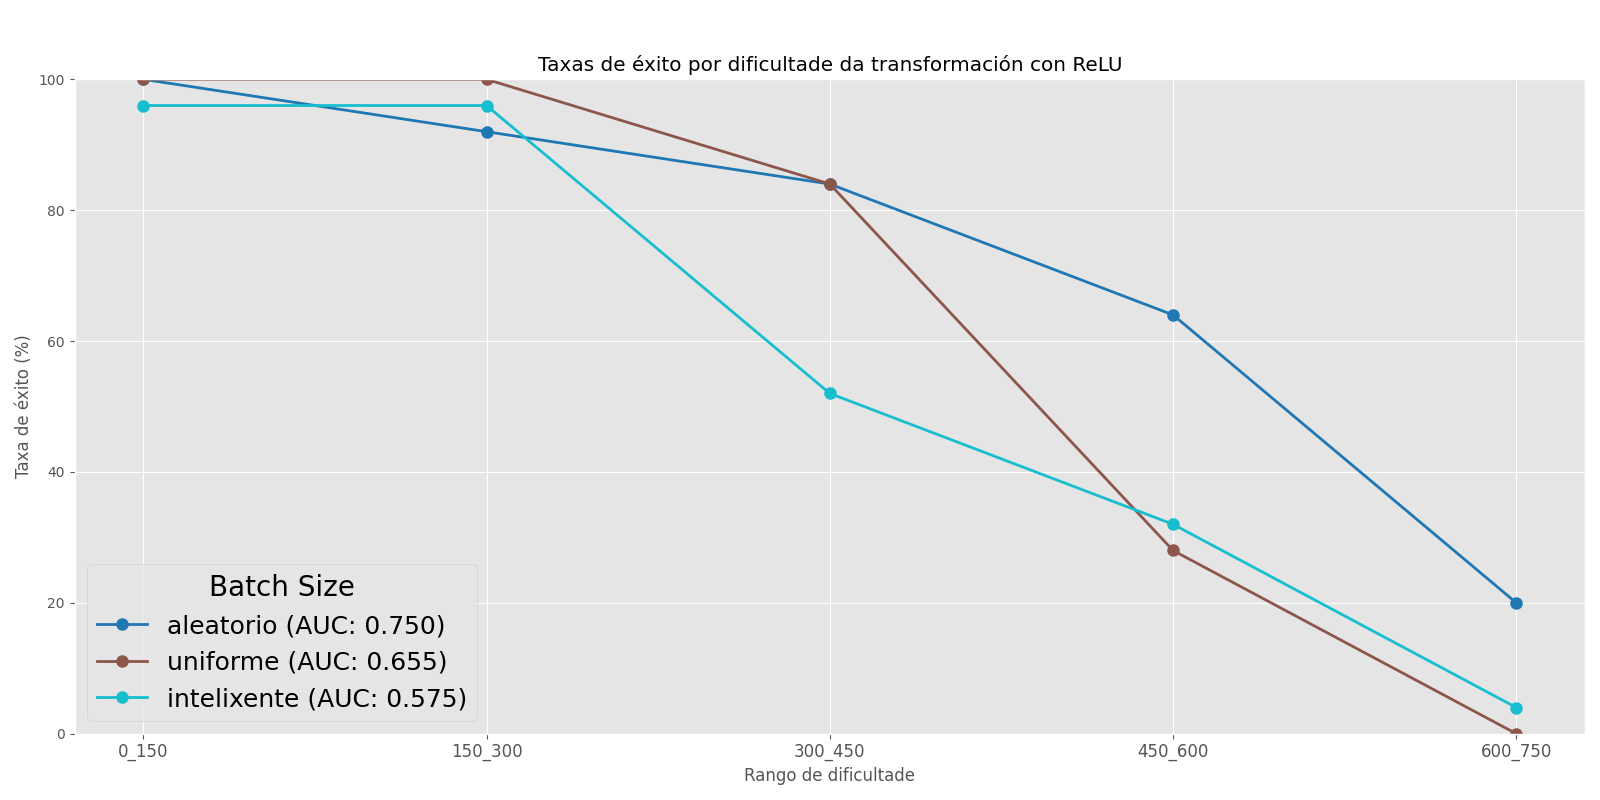
\includegraphics[width=\textwidth]{imaxes/muestraje/experiment_plot_RFMID_st_relu.png}
        \caption{Función de activación ReLU}
        \label{fig:sampling_types_relu}
    \end{subfigure}\hfill
    \begin{subfigure}[b]{0.48\textwidth}
        \centering
        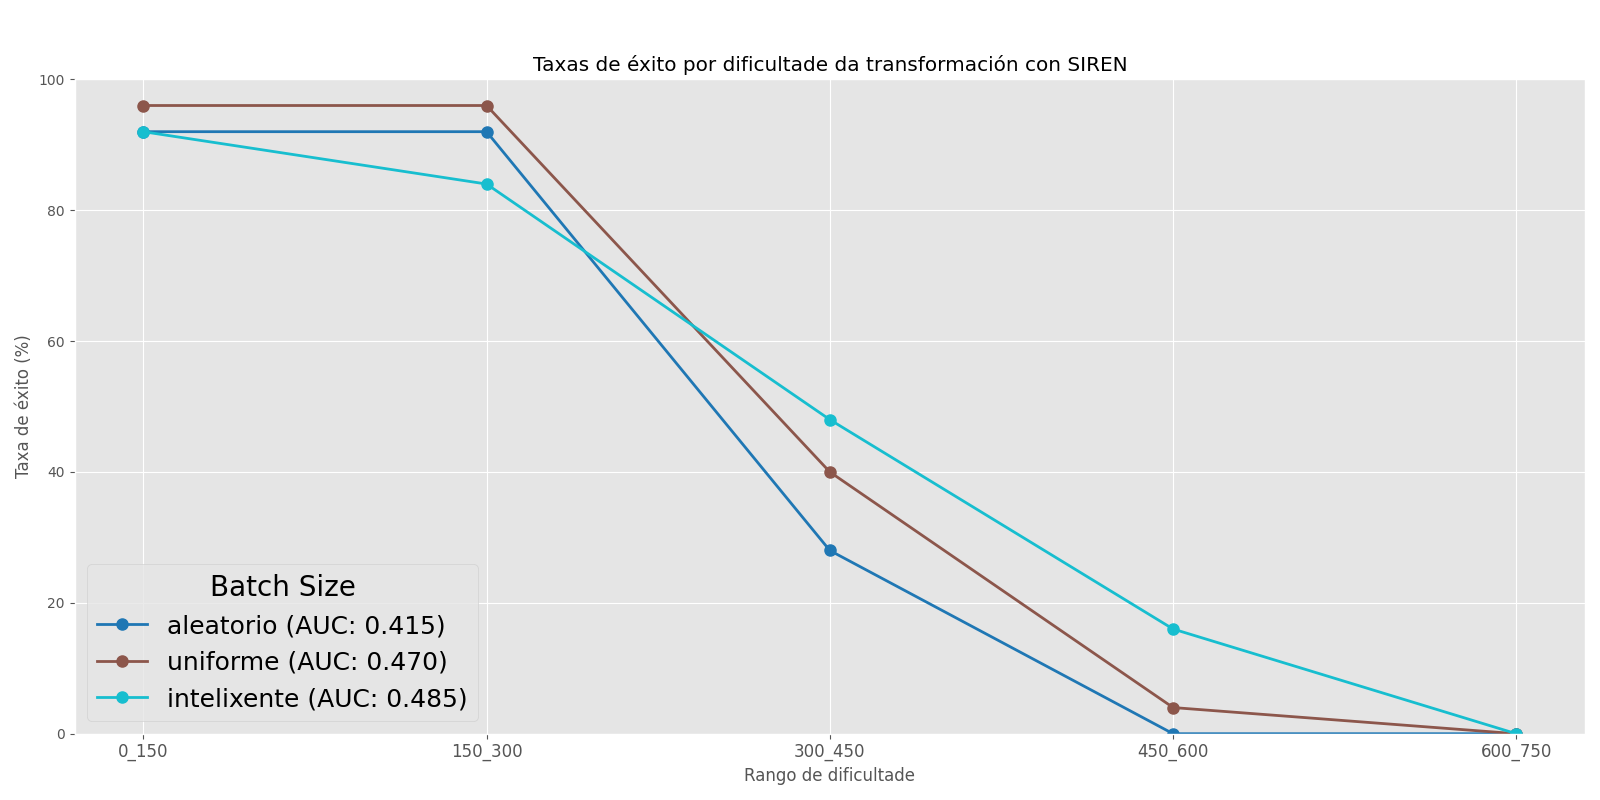
\includegraphics[width=\textwidth]{imaxes/muestraje/experiment_plot_RFMID_st_SIREN.png}
        \caption{Función de activación SIREN}
        \label{fig:sampling_types_siren}
    \end{subfigure}
    \caption{Comparación de las diferentes estrategias de muestreo sobre imágenes del dataset RFMID}
    \label{fig:sampling_types_comparisons}
\end{figure}

\subsection{Discusión}
\label{subsec:Discusion-sampling}

La hipótesis de la estrategia de muestreo inteligente no parece ser adecuada, con resultados similares a la estrategia aleatoria. 
Lo mismo ocurre con la estrategia uniforme.

Igual que en experimentos anteriores, la función de activación ReLU parece dar mejores resultados que SIREN con RFMID, especialmente con mayores dificultades de transformación.

\subsection{Conclusiones}
\label{subsec:Conclusions-sampling}
Se concluye que, en contra de la hipótesis inicial, las estrategias de muestreo implementadas, como la ponderada por el contenido de la imagen, no aportan una mejora significativa en el rendimiento del registro en comparación con el muestreo aleatorio estándar. Esto sugiere que la información relevante para la deformación está lo suficientemente bien distribuida como para que un muestreo aleatorio sea capaz de capturar los puntos necesarios para la convergencia, siempre que el tamaño de lote sea adecuado.

\section{Inicialización}
\label{sec:Inicialización}

\subsection{Planteamiento}
\label{subsec:Planteamento-initialization}

Es posible que la inicialización de la red sea un factor clave, y que ciertos desplazamientos iniciales provoquen que la red sea incapaz de aprender la transformación correcta, o que le cueste mucho más aprenderla.

Para validar esta hipótesis se implementó una lotería de inicialización, donde se utiliza la pérdida en la época 0 para determinar la inicialización de la red más beneficiosa sobre la que seguir entrenando.

\begin{figure}[tbp]
    \centering
    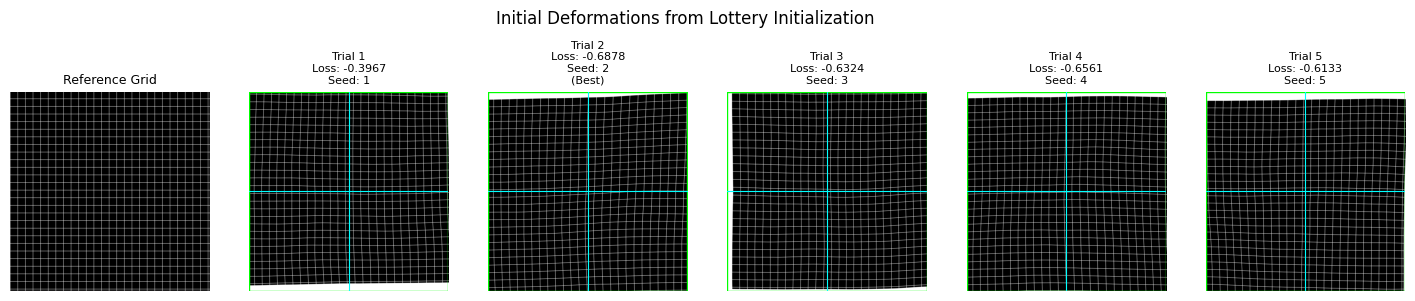
\includegraphics[width=0.8\textwidth]{imaxes/lottery/initial_deformations_combinedMLP.png}
    \caption{Ejemplos de las diferentes inicializaciones con la función de activación RELU}
    \label{fig:lottery_initial_deformations_combinedMLP}
\end{figure}

\begin{figure}[tbp]
    \centering
    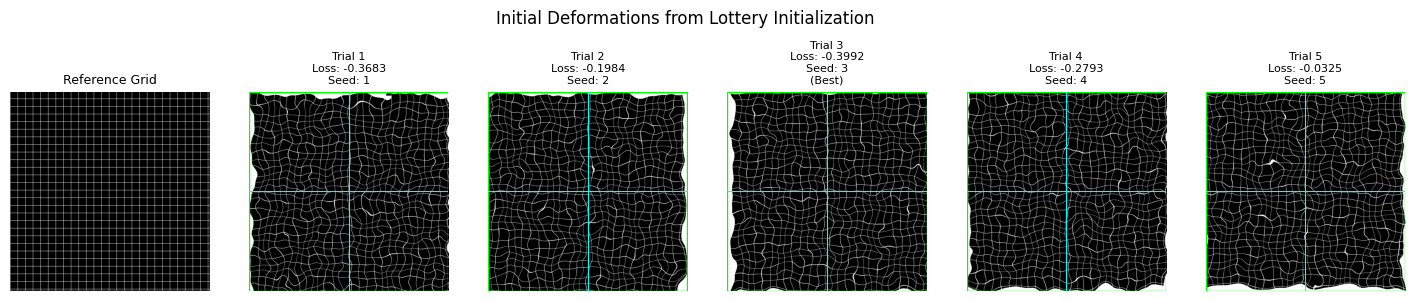
\includegraphics[width=0.8\textwidth]{imaxes/lottery/initial_deformations_combinedSIREN.png}
    \caption{Ejemplos de las diferentes inicializaciones con la función de activación SIREN}
    \label{fig:lottery_initial_deformations_combinedSIREN}
\end{figure}

\subsection{Resultados}
\label{subsec:Resultados-initialization}

En la figura \ref{fig:lottery} se muestran los resultados de diferentes valores de la lotería de inicialización.

\begin{figure}[tbp]
    \centering
    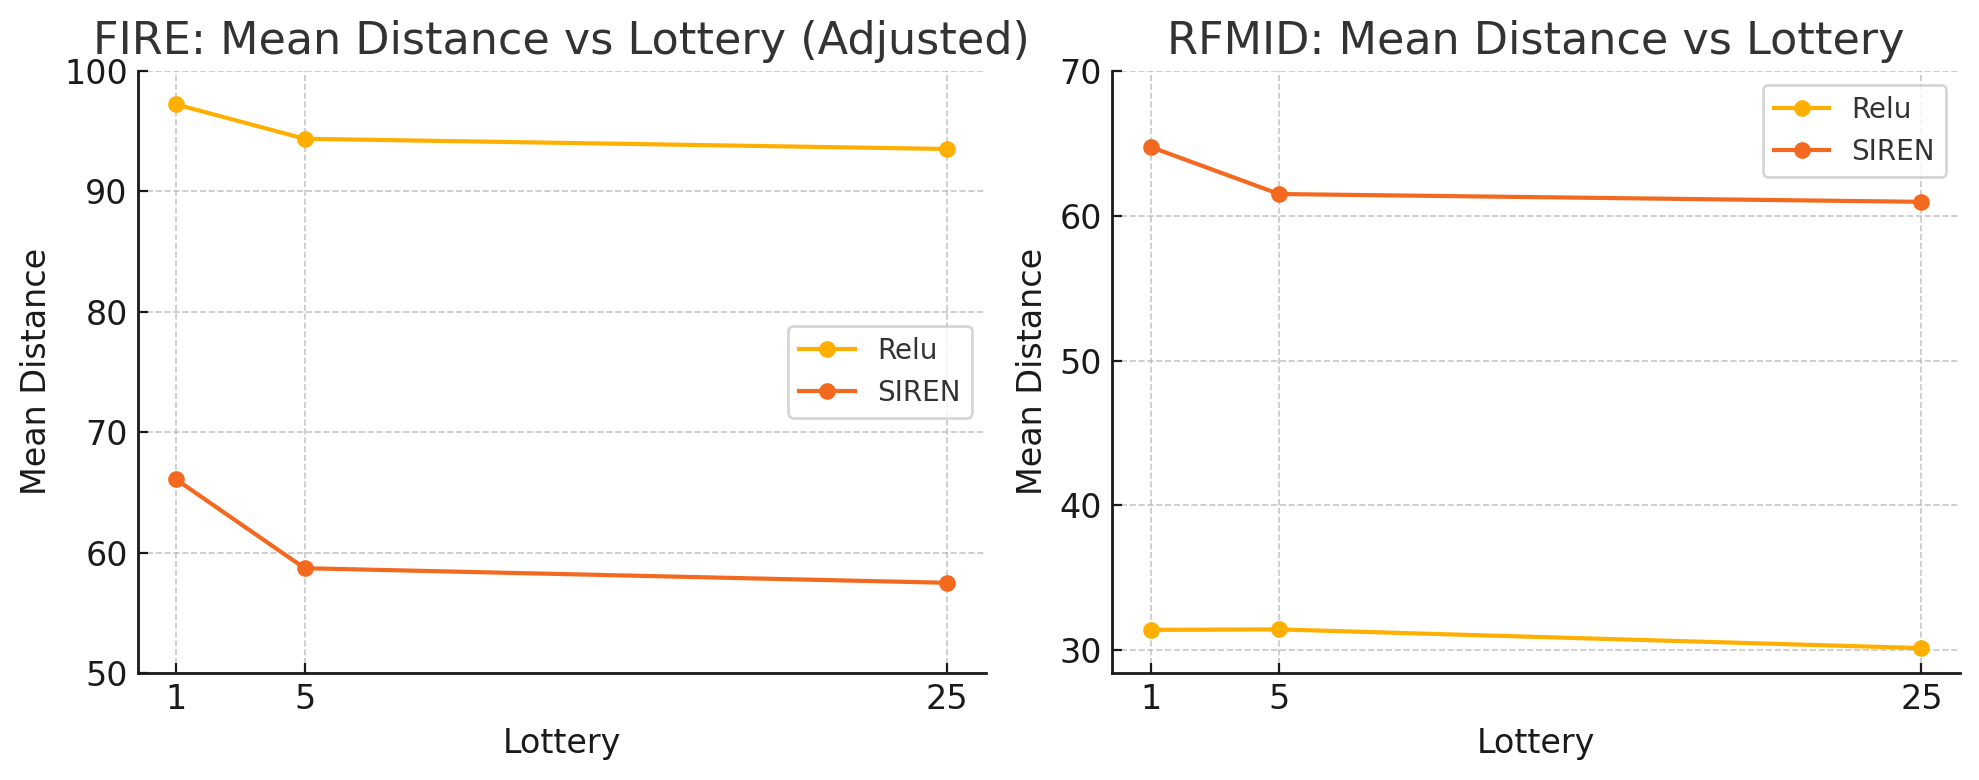
\includegraphics[width=0.8\textwidth]{imaxes/lottery/lotery.png}
    \caption{Resultados de la lotería de inicialización}
    \label{fig:lottery}
\end{figure}

\subsection{Discusión}
\label{subsec:Discusion-initialization}

La inicialización estándar de SIREN propuesta por Sitzmann et al. \cite{sitzmann2020implicitneuralrepresentationsperiodic} fue diseñada para tareas de reconstrucción de imágenes, y no necesariamente para regresión de campos de deformación.
Esto puede provocar que el proceso de optimización dedique mucho tiempo a contrarrestar una mala inicialización.

\subsection{Conclusiones}
\label{subsec:Conclusions-initialization}

Se observa que la lotería de inicialización sí que provoca mejoras en el rendimiento de la red, aunque no muy significativas, y no se beneficia particularmente de utilizar más de 5 inicializaciones.
Es posible que fuera mejor esperar hasta una iteración algo más avanzada para determinar la inicialización, ya que en la época 0 no hay ninguna seguridad de que no sea un mínimo local, pero esto también implicaría un mayor coste computacional.

Una posible mejora a la lotería de inicialización sería utilizar un número mayor de épocas antes de determinar la inicialización ganadora, ya que la pérdida inicial no es necesariamente representativa del rendimiento final de la red.
De la misma forma, sería interesante comparar diferentes estrategias de inicialización, como la inicialización gaussiana o la inicialización uniforme, para determinar si alguna de ellas proporciona una ventaja significativa sobre la inicialización estándar de SIREN.

\section{Ajuste dinámico del tamaño de lote}
\label{sec:Dynamic tamaño de lote}

\subsection{Planteamiento}
\label{subsec:Planteamento-phases}

Se teoriza que la red puede beneficiarse de dividir el proceso de registro en diferentes fases, donde inicialmente se utiliza un tamaño de lote reducido para aprender la transformación global, y posteriormente se aumenta el tamaño de lote para aprender las transformaciones locales.
Para esto utilizaremos la estrategia de muestreo uniforme, que permite asegurar que se cubre toda la imagen con la misma densidad, lo que es más importante con tamaños de lote pequeños. El learning rate se modifica de forma proporcional para mantener la relación entre este y el tamaño de lote.

\subsection{Resultados}
\label{subsec:Resultados-phases}

Los resultados de utilizar diferentes números de fases se pueden observar en la figura \ref{fig:nphases}.
\begin{figure}[tbp]
    \centering
    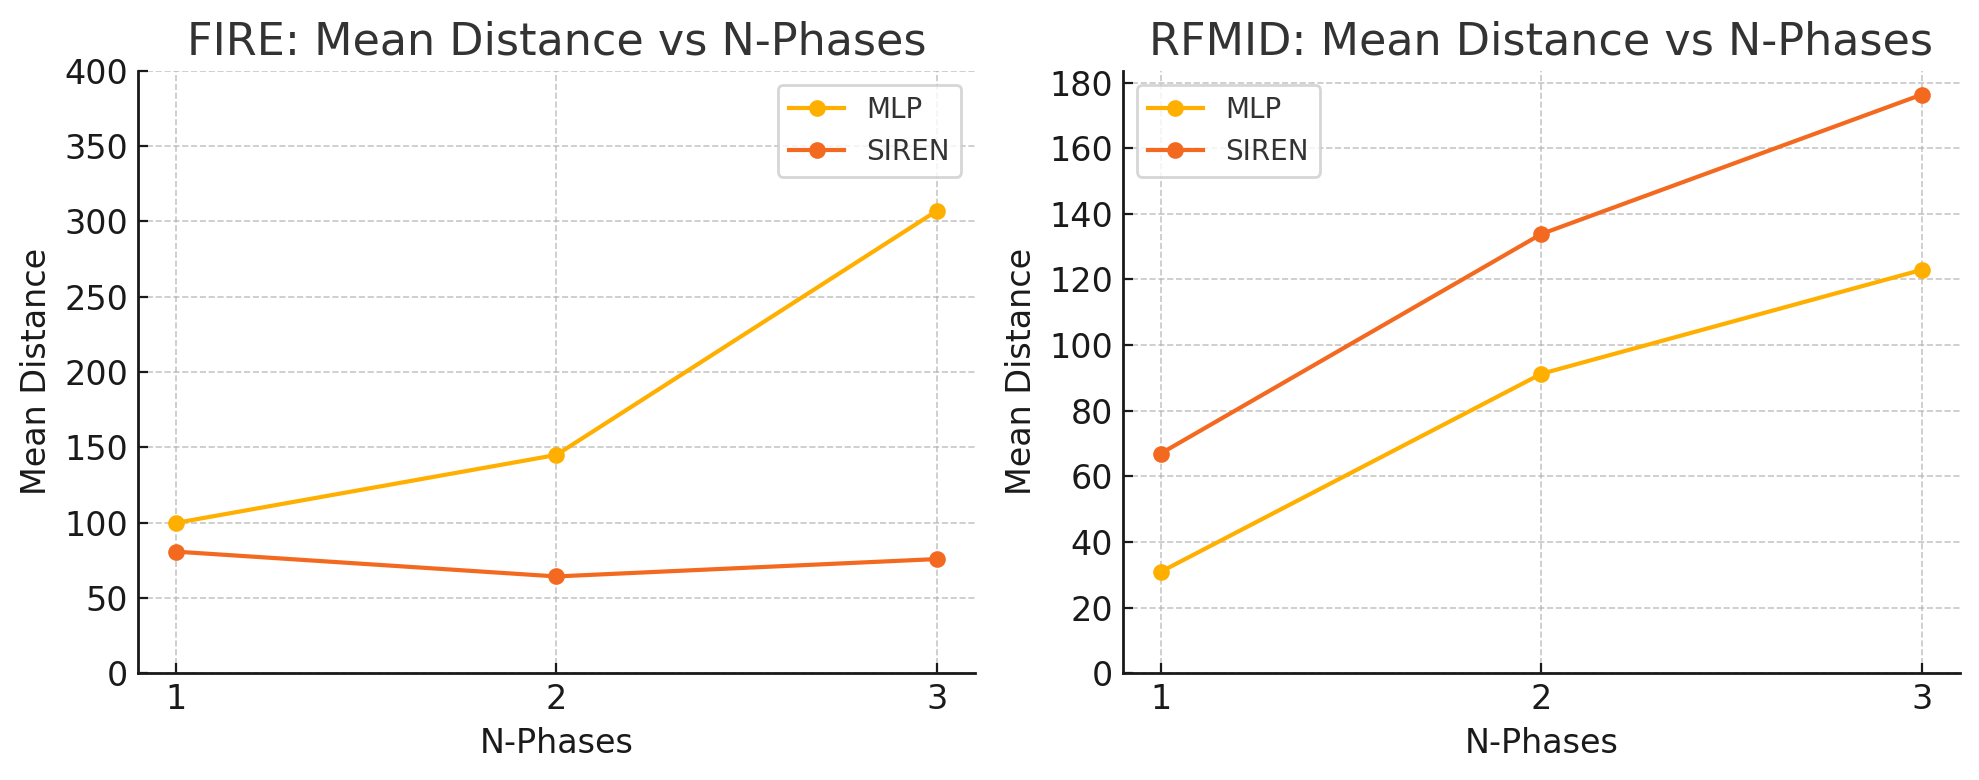
\includegraphics[width=0.8\textwidth]{imaxes/lottery/nphases.png}
    \caption{Resultados de usar distinto número de fases}
    \label{fig:nphases}
\end{figure}

\subsection{Discusión}\label{subsec:Discusion-phases}

Los resultados presentados en la figura \ref{fig:nphases} muestran una tendencia clara y contraria a la hipótesis inicial, ya que el rendimiento de la red empeora progresivamente a medida que se incrementa el número de fases. La estrategia de comenzar con un tamaño de lote pequeño para aprender la transformación global antes de refinar los detalles con un tamaño de lote mayor resulta ser contraproducente.

Una posible explicación es que la idea de que un lote pequeño favorece el aprendizaje global es incorrecta en este contexto. Un tamaño de lote reducido ofrece una estimación muy ruidosa y poco representativa, lo que puede llevar el entrenamiento por un camino inestable e impedir que la red converja hacia una buena solución global en la fase inicial. En cambio, un tamaño de lote grande y constante, como se validó en la sección \ref{sec:Tamaño de lote}, proporciona desde el principio información suficiente tanto a nivel global como local, permitiendo que la red aprenda ambas transformaciones simultáneamente de forma más estable y eficaz.

Por lo tanto, la estrategia de dividir el entrenamiento en fases no solo no aporta beneficios, sino que resulta perjudicial al introducir inestabilidad en las etapas cruciales del aprendizaje. Este experimento refuerza la conclusión de que un tamaño de lote grande es fundamental para el éxito del registro con esta metodología.

\subsection{Conclusiones}
\label{subsec:Conclusions-phases}

Se concluye que la estrategia de ajuste dinámico del tamaño de lote es ineficaz y perjudicial para esta tarea. La inestabilidad introducida en las fases iniciales del entrenamiento anula cualquier posible beneficio teórico de aprender las transformaciones por etapas. La red demuestra ser más robusta y eficaz cuando se entrena con un tamaño de lote grande y constante desde el principio, confirmando que este enfoque es superior para aprender simultáneamente las características globales y locales de la deformación.

% \FloatBarrier

\section{Comparativa y resumen de resultados}
\label{sec:Comparativa e resumo}

Tras la realización de los experimentos descritos anteriormente, se pueden extraer las siguientes conclusiones:

\subsection{Rendimiento por dataset}
\label{subsec:Rendemento por dataset}

\textbf{Dataset FIRE:} El rendimiento en el dataset FIRE, que contiene imágenes reales de retina, es significativamente más bajo que en el dataset RFMID. La categoría P resulta imposible de registrar debido al bajo grado de superposición (<75\%). Las categorías S y A muestran tasas de éxito alrededor del 20\%, siendo la categoría S ligeramente superior.

\textbf{Dataset RFMID:} El rendimiento en el dataset RFMID es considerablemente mejor, especialmente para transformaciones de baja complejidad (norma de Frobenius 0-150), donde se alcanza un éxito del casi 100\%. El rendimiento decae progresivamente con la complejidad de la transformación.

\subsection{Comparación de funciones de activación}
\label{subsec:Comparación de funcións de activación}

Los resultados muestran una clara diferenciación entre las funciones de activación según el tipo de dataset:

\textbf{ReLU:} Muestra un rendimiento superior en el dataset RFMID, debido a su capacidad natural para aprender transformaciones lineales.

\textbf{SIREN:} Aunque teóricamente más adecuada para aprender transformaciones complejas, tiene dificultades para representarlas adecuadamente. Tiende a transformaciones locales y poco realistas y si no se regulariza adecuadamente, converge a mínimos locales no deseados.

\subsection{Impacto de los parámetros principales}
\label{subsec:Impacto dos parámetros principais}

\textbf{Función de pérdida:} Las métricas basadas en características estructurales (NCC, SSIM) son superiores para imágenes reales con variabilidad de iluminación (FIRE), mientras que las métricas basadas en píxeles (L1, MSE) son más efectivas para imágenes sin variabilidad (RFMID).

\textbf{Regularización:} La regularización hiperelástica es la más relevante para evitar deformaciones no realistas. El valor óptimo depende del par de imágenes concreto a registrar. SIREN requiere valores más altos que ReLU ya que tiene una mayor tendencia al sobreajuste.

\textbf{Tamaño de lote:} Constituye uno de los parámetros más críticos. Valores mayores (10000-50000) proporcionan mejores resultados que tamaños pequeños (1000), aunque el beneficio decrece para valores muy altos (>50000).

\textbf{Resolución:} No se observan beneficios significativos por encima de 1000×1000 píxeles, sugiriendo que la información relevante para el registro ya está capturada en resoluciones moderadas.

\subsection{Limitaciones identificadas}
\label{subsec:Limitacións identificadas}

\textbf{Complejidad de las transformaciones:} El factor limitador principal es la complejidad de las transformaciones. Tanto ReLU como SIREN muestran dificultades con las transformaciones de alta complejidad, independientemente de la optimización de parámetros.

\textbf{Superposición de imágenes:} La baja superposición entre imágenes (categoría P de FIRE) dificulta enormemente el registro, sugiriendo que las redes implícitas requieren un mínimo de información compartida.

\textbf{Estrategias de muestreo:} Contrario a lo esperado, las estrategias inteligentes de muestreo (ponderadas por contenido) no muestran beneficios sobre el muestreo aleatorio, sugiriendo que la información relevante está distribuida de forma más uniforme de lo esperado.

\subsection{Conclusiones generales}
\label{subsec:Conclusións xerais}

La fase experimental de este trabajo, centrada en la adaptación y evaluación de un marco basado en representación neuronales implícitas para la tarea de registro de imágenes oftalmológicas, demuestra que las redes implícitas son aplicables al registro de imágenes de retina, pero con limitaciones importantes. El rendimiento depende críticamente de la complejidad de las transformaciones y del grado de superposición entre imágenes. Aunque los resultados son prometedores para casos de complejidad baja a moderada, el registro de imágenes con transformaciones complejas o baja superposición sigue siendo un desafío que requiere investigación adicional.

Si bien el rendimiento actual no es óptimo, las comparaciones con otras metodologías de registro del estado del arte deben tener en cuenta que la mayoría de ellas integran conocimiento específico del dominio frente al método aquí presentado, que funciona de forma general aprendiendo a partir de los píxeles. Esto sugiere futuras líneas de investigación que combinen las ventajas de las redes implícitas con conocimientos específicos del dominio, como la anatomía de la retina o las características de los vasos sanguíneos, para mejorar el rendimiento en registros complejos. El análisis de las limitaciones del modelo y exploración de diferentes estrategias proporcionan una base sólida para futuras investigaciones en el campo.